\chapter{J/$\Psi$ Transverse Spin Dependent Phenomena}
\label{ch::jpsi}
\ifpdf
\graphicspath{{Chapters/JPsi/Figs/}}
\fi

This chapter describes the analysis performed in the intermediate invariant mass
range at COMPASS.  The biggest advantage about the intermediate mass range is an
increase in statistics.  The intermediate mass range for this thesis is defined
as 2.5-4.3~{\gvcw}.  The intermediate mass range contains approximately 1.6
times more events than the high mass range above 4.3~{\gvcw}.  On the other
hand, the intermediate mass range results from several reactions.  Nevertheless,
{\jp} production is by far the most dominant reaction and therefore the this
chapter assumes the results are from the {\jp} reaction.  A theoretical
introduction related to transverse {\jp} spin asymmetries is provided in
Sec~\ref{sec::theory_jpsi}.  As of yet, the exact mechanism for J/$\Psi$
production is unknown and therefore the exact {\jp} vertex coupling is unknown.
Nevertheless, the analysis techniques in this chapter contribute to the
transverse spin knowledge of J/$\Psi$ production.  The reaction of
interest is
\begin{equation}
  \pi^-(P_a) + P(P_b, S_T) \rightarrow J/\Psi + X \rightarrow \mu^-(\ell) +
  \mu^+(\ell') + X,
\end{equation}
\noindent
where the proton target, $P$, is transversely polarized with spin $S_T$.

The dimuon final state from {\jp} production is indistinguishable from the
Drell-Yan dimuon final state described the previous analyses in
chapter~\ref{ch::hmanalysis}.  For this reason, similar event selection and data
quality are used to study the dimuon production resulting from {\jp} decays.  On
the other hand, the {\jp} production has a higher background percentage from
Drell-Yan and other components to be taken into account.  The results presented
in this chapter are determined from the left-right asymmetry analysis as in
Sec~\ref{sec::leftrightasym}, where again the left-right asymmetry is defined as

\begin{equation}
  A_{lr} = \frac{1}{|S_T|}
  \frac{\sigma_l - \sigma_r}{\sigma_l +
    \sigma_r}.
\end{equation}

\subsection{Data Collection and Event Selection}
The data collection is described in Sec~\ref{sec::datacollection} and the data
stability tests are described in Sec~\ref{sec::stability}.  Both the Drell-Yan
analysis and the {\jp} production analysis study dimuon final states so the
spectrometer data taking conditions are the same.  In particular the measurement
in this chapter results from a 190~{\gvc} $\pi^-$ beam impinged on a
transversely polarized NH$_3$ target from the 2015 COMPASS spectrometer data
taking conditions.

The event selection in this chapter is similar to the event selection in the
previous chapter, Sec~\ref{sec::dy_eventselection}.  The cuts are chosen to
ensure two oppositely polarized muons are detected with a vertex in the
transversely polarized NH$_3$ target.  Sec~\ref{sec::dy_eventselection}
describes the cut selection and the reason for each cut.  The only event
selection difference, from Sec~\ref{sec::dy_eventselection}, is the selected
invariant mass.  The nominal {\jp} invariant mass and width are 3.096~{\gvcw}
and 92.9$\times10^{-6}$~{\gvcw} respectively~\cite{Tanabashi:2018oca}.
Therefore to ensure the events for this analysis result from {\jp} production,
the analysis invariant mass range should be where the {\jp} signal to background
is highest.  This is in contrast to the Drell-Yan analyses which required the
invariant mass to be above 4.3~{\gvcw}.

\subsubsection{{\jp} Invariant Mass Range}\label{sec::jpMassRange}
The COMPASS spectrometer has a finite mass resolution which therefore means the
events resulting from {\jp} production have an invariant mass spread larger than
the nominal {\jp} width.  For this reason the cut on invariant mass should be a
range much larger than the nominal {\jp} width.
Fig.~\ref{fig::DY_InvariantMassJPsi} shows the 2015 dimuon invariant mass
distribution and the other production components around the {\jp} invariant
mass.

\begin{figure}[h!t]
  \centering 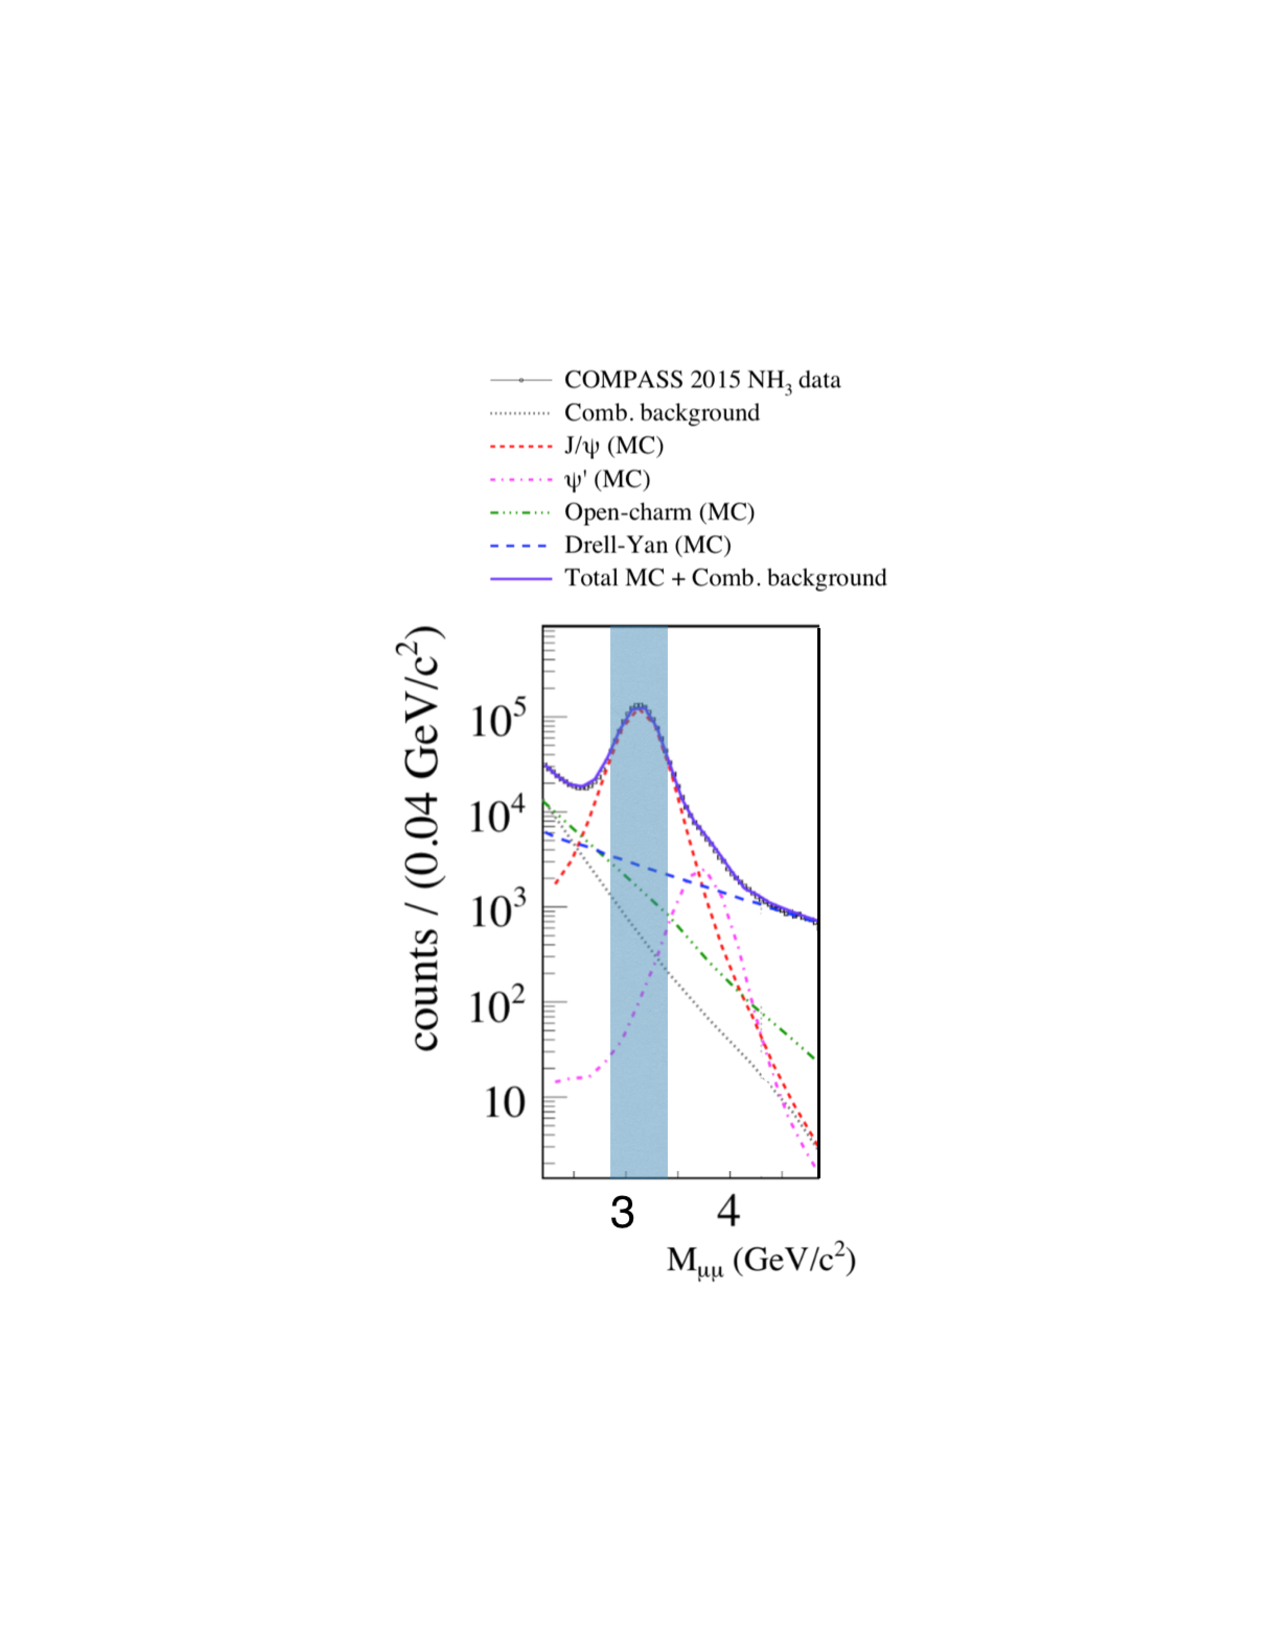
\includegraphics[width=0.3\textwidth,trim=6cm 6cm 6cm 5.5cm,
    clip]{DY_InvariantMassJPsi}
  \caption{The 2015 COMPASS invariant dimuon mass distribution and a fit to this
    data.  The data fit is from Monte-Carlo and combinatorial background
    analysis and is provided to show the background processes.  The shaded blue
    region shows the analysis mass range for the analysis in this chapter.  This
    image is taken from~\cite{compassDYpaper}.}
  \label{fig::DY_InvariantMassJPsi}
\end{figure}

As can be seen in Fig.~\ref{fig::DY_InvariantMassJPsi}, regardless of the
analysis mass range chosen, there are still events resulting from the other
background processes.  The normalized systematic variance resulting from
background processes is derived in Appendix~\ref{app::sysEventContam} as

\begin{equation}
  \frac{\sigma^2_{systematic}}{\sigma^2_{statistical}} = \frac{(1-p)^2}{p^2},
\end{equation}
\noindent
and the total variance from statistical fluctuations and background
contributions is
\begin{equation}
  \delta^2 A_{lr,J/\Psi} = \frac{(1-p)^2 + 1}{p^2}\sigma^2_{statistical},
  \label{equ::JPerrorTot}
\end{equation}
where $p$ is the {\jp} purity.  Therefore the analysis invariant mass range
should have a {\jp} purity as high as possible to reduce the systematic error
while still including as much data as possible to reduce the statistical error.
The total error however, is dominated by statistical error for any purity larger
than 50\%.  That being the case, Eq.~\ref{equ::JPerrorTot} is derived assuming
$(1-p)$ is small and therefore a desired purity of 90\% or greater was chosen to
safely ensure Eq.~\ref{equ::JPerrorTot} is valid.

The {\jp} purity as a function of mass range is determined from a Monte-Carlo
data set.  The same Monte-Carlo described in Table~\ref{tab::MCproduction} was
used to calculate the {\jp} purity.  In particular the processes included are
Drell-Yan production, open charm production, $\Psi$' production and {\jp}
production.  To determine the purity, the real data is fit using the Monte-Carlo
data which determines the counts from each process.  The Monte-Carlo fit is
accomplished by normalizing the invariant mass distribution from each
Monte-Carlo sample and then fitting using the sum of the four normalized
distributions to fit the real data.  The fit function is defined as
\begin{align}
  F_{J/\Psi \;Fit}(x) = &N_{J/\Psi}h_{J/\Psi}(x) + N_{Drell-Yan}h_{Drell-Yan}(x)
  \\ \nonumber
  &+ N_{Open\;Charm}h_{Open\;Charm}(x)+N_{\Psi'}h_{\Psi'}(x),
\end{align}
\noindent
where $h(x)$ represents the number of counts from the normalized histogram
distribution and the $N$'s are the fit parameters.  Fig.~\ref{fig::MC_NormInvM}
shows the four normalized Monte-Carlo invariant mass distributions and
Fig.~\ref{fig::MC_fitQt} shows the Monte-Carlo fit to the real data in one $q_T$
bin.

\begin{figure}[h!t]
  \centering
  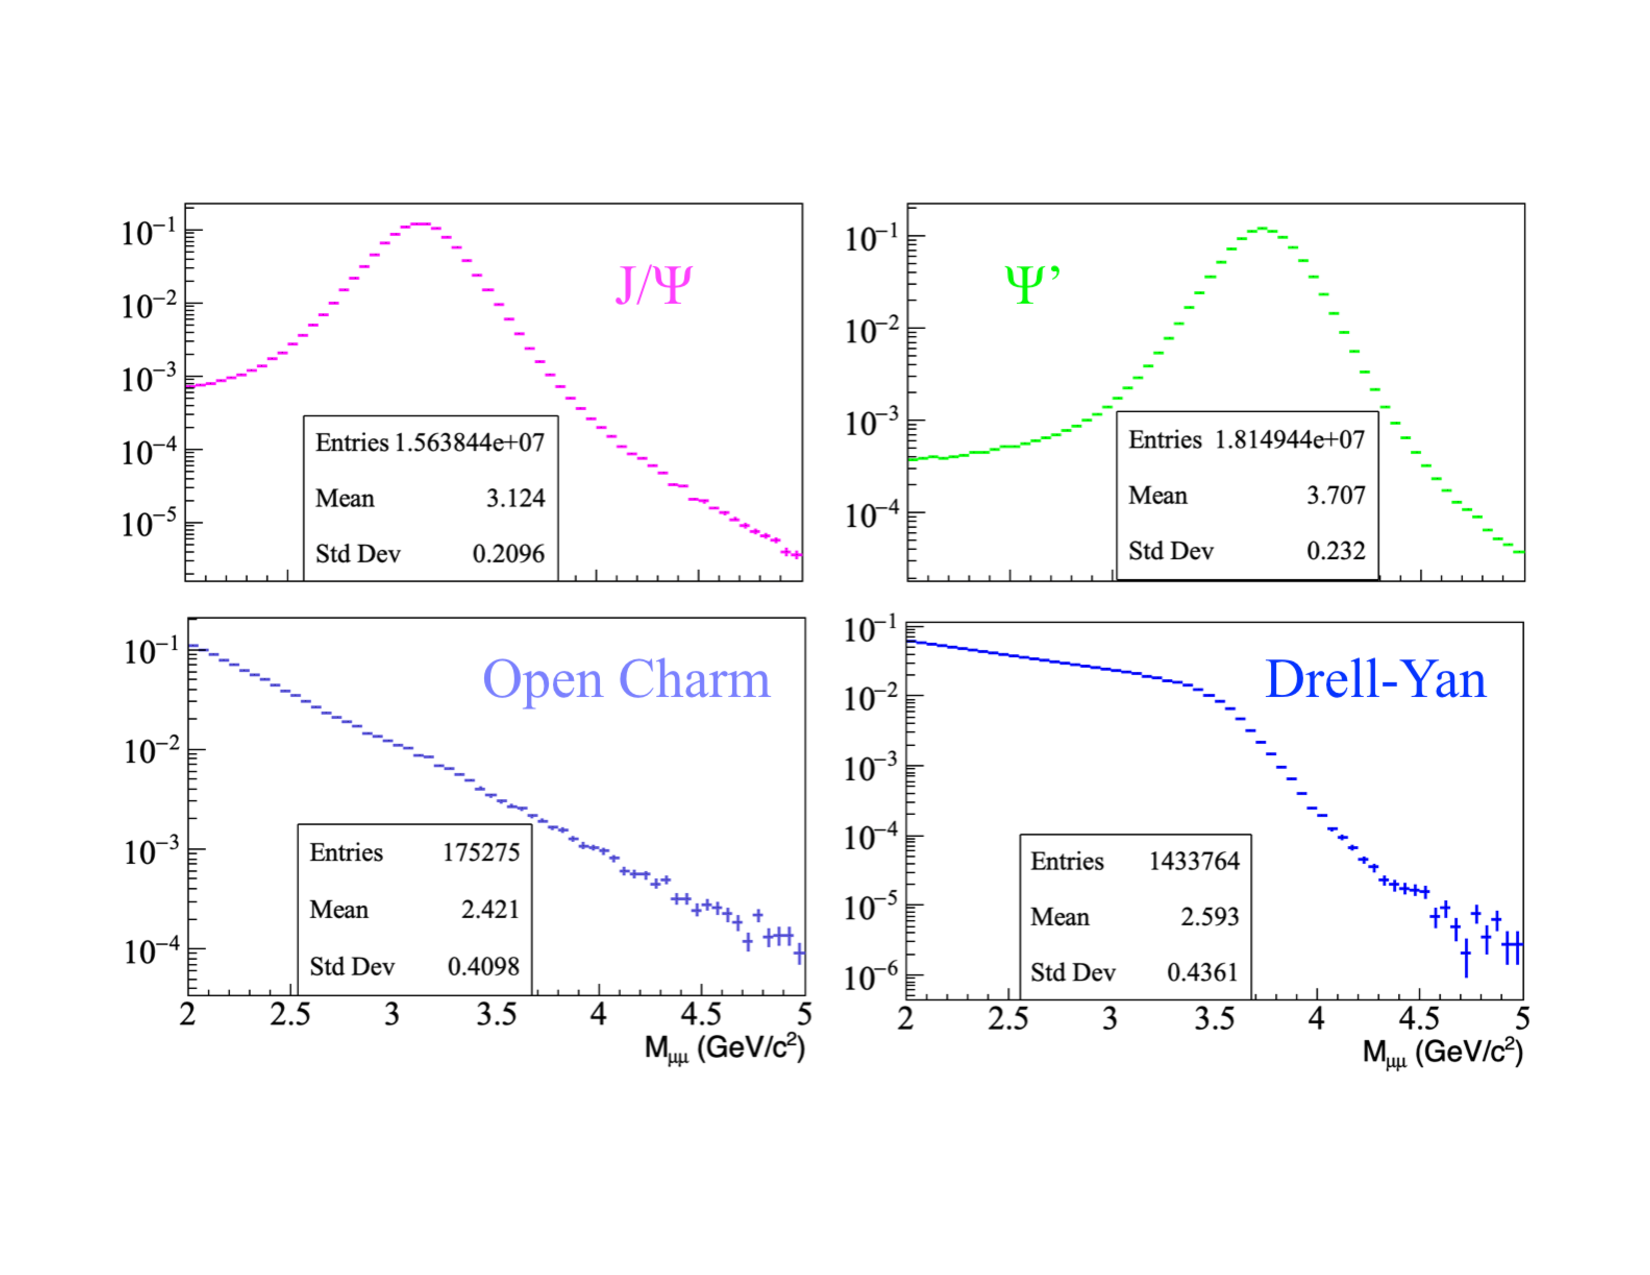
\includegraphics[width=0.8\textwidth, trim=2cm 3cm 2cm 3cm, clip]{MC_NormInvM}
  \caption{The normalized invariant mass distributions from the four simulated
    Monte-Carlo processes.  These distributions are used to fit the real data.}
  \label{fig::MC_NormInvM}
\end{figure}

\begin{figure}[h!t]
  \centering
  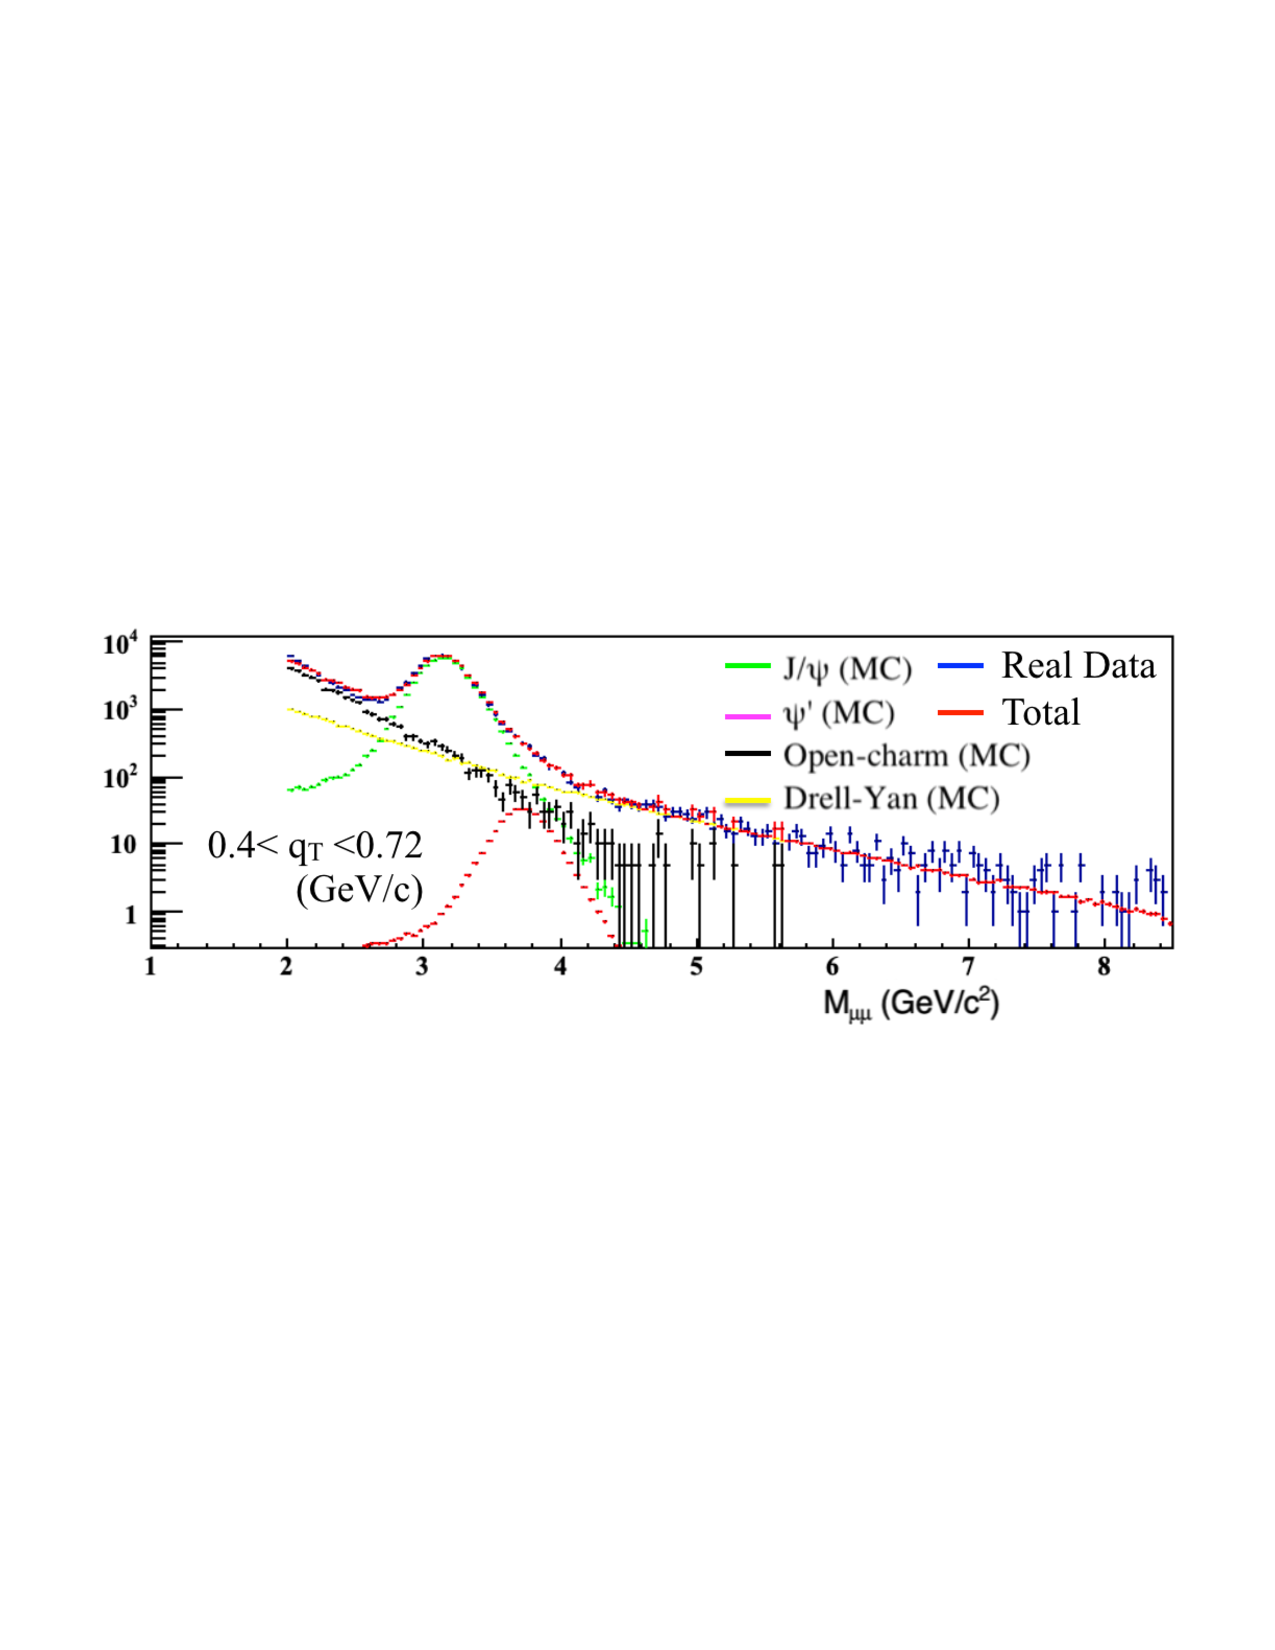
\includegraphics[width=0.8\textwidth, trim=1cm 10cm 1cm 10cm, clip]{MC_fitQt}
  \caption{An example of the Monte-Carlo fit to real data in one $q_T$ bin of
    the real data.  This fit is used to determine the distribution of {\jp}
    purity.}
  \label{fig::MC_fitQt}
\end{figure}

Once the fits are performed, the {\jp} purity in each invariant bin is
determined as

\begin{equation}
  p(x) = \frac{N_{J/\Psi}h_{J/\Psi}(x)}{N_{J/\Psi}h_{J/\Psi}(x) + N_{Drell-Yan}h_{Drell-Yan}(x) N_{Open\;Charm}h_{Open\;Charm}(x)+N_{\Psi'}h_{\Psi'}(x)}.
\end{equation}
\noindent
Table~\ref{tab::JPsiPurity} summarizes the {\jp} purity as a function of the
mass range.  For this analysis an invariant mass range of 2.87-3.38~{\gvcw} was
chosen to safely have a {\jp} purity of 90\% or greater.
Tables~\ref{tab::JPsiStats1}-~\ref{tab::JPsiStats2} summarizes the number of
events remaining after each cut.

\begin{table}
  \centering
  \begin{tabular}{ |c|c| }
    \hline
    \textbf{Mass range GeV/c$^2$}& \textbf{{\jp} Purity \%}
    \\ \hline \hline
    2.5-4.3& 79.7 $\pm$ 2.9 \\ \hline
    2.78-3.46& 88.9 $\pm$ 2.0 \\ \hline
    \textbf{2.87-3.38}& \textbf{91.3 $\pm$ 1.5} \\ \hline
    2.95-3.29& 92.9 $\pm$ 1.0 \\ \hline
    3.08-3.17& 94.0 $\pm$ 1.0 \\ \hline
    
  \end{tabular}
  \caption{{\jp} purity as a function of the invariant mass range}
  \label{tab::JPsiPurity}
\end{table}

\begin{table}[h!t]
  \begin{tabular}{ |c|c|c|c|c|c| }
    \hline \textbf{Cuts}& \textbf{W07}& \textbf{W08}& \textbf{W09}&
    \textbf{W10}& \textbf{W11} \\ \hline

    \multirow{3}{9em}{$\mu^-\mu^+$ 2-8.5 GeV/c$^2$ with a common best primary
      vertex}& & & & & \\
    & 1,573,372& 1,572,255& 1,620,593& 1,683,263& 2,598,485\\
    & & & & & \\ \hline
    
    Good Spills& 1,298,306& 1,223,877& 1,333,335& 1,374,620& 1,901,071
    \\ \hline
    
    0$<$ x$_{\pi}$ x$_N$ $<$1, -1$<$ x$_F$ $<$1& 1,298,278& 1,223,851&
    1,333,307& 1,374,599& 1,901,033 \\ \hline

    0.4$<$ q$_T$ $<$5(GeV/c)& 1,121,908& 1,056,835& 1,151,253& 1,187,125&
    1,641,463\\ \hline

    Z Vertex within NH$_3$& 314,965& 298,531& 324,413& 335,659& 465,172
    \\ \hline

    Vertex Radius $<$ 1.9cm& 308,278& 292,114& 317,985& 328,658& 455,580
    \\ \hline

    2.87$< M_{\mu\mu} <$3.38 (GeV/c$^2$)&
    170,041& 160,450& 174,696& 180,795& 250,921
    \\ \hline
    
  \end{tabular}
  \caption{Selected dimuon events for the first five data periods from the
    intermediate mass range analysis of 2015 COMPASS data}
  \label{tab::JPsiStats1}
\end{table}

\begin{table}[h!t]
  \begin{tabular}{ |c|c|c|c|c|c|c| }
    \hline \textbf{Cuts}& \textbf{W12}& \textbf{W13}& \textbf{W14}&
    \textbf{W15} & \textbf{WAll} & \textbf{Remaining} \\ \hline

    \multirow{3}{9em}{$\mu^-\mu^+$ 2-8.5 GeV/c$^2$ with a common best primary
      vertex}& & & & & & \\
    &1,932,425& 1,680,706& 1,094,525& 640,095& 14,395,719&
    100.00 \% \\ & & & & & & \\ \hline

    Good Spills& 1,659,030& 1,314,489& 982,131& 616,734& 11,703,593&
    81.3 \% \\ \hline

    0$<$ x$_{\pi}$ x$_N$ $<$1, -1$<$ x$_F$ $<$1&
    1,658,996& 1,314,470& 982,125& 616,720& 11,703,379&	81.3 \% \\ \hline

    0.4$<$ q$_T$ $<$5(GeV/c)&
    1,432,115& 1,134,223& 846,897& 532,045& 10,103,864&	70.2 \% \\ \hline

    Z Vertex within NH$_3$&
    406,975& 322,964& 241,673& 151,937&	2,862,289& 19.9  \% \\ \hline

    Vertex Radius $<$ 1.9cm&
    398,610& 316,149& 236,019& 148,834& 2,802,227& 19.5  \% \\ \hline

    2.87$< M_{\mu\mu} <$3.38 (GeV/c$^2$)&
    219,110& 173,701& 129,346& 81,808& 1,540,868& 10.7  \% \\ \hline
    
  \end{tabular}
  \caption{Selected dimuon events for the last four data periods and the total
    number of events from the intermediate mass range analysis of 2015 COMPASS
    data}
  \label{tab::JPsiStats2}
\end{table}


\subsection{Binning}

The analysis is determined as a function of the variables $x_N$, $x_{\pi}$,
$x_F$, $q_T$ and $M_{\mu\mu}$.  These are the same variables used to bin the
high mass Drell-Yan analysis.  The left-right asymmetry analysis is binned in
each of the kinematic variables by requiring an equal amount of data per
kinematic bin.  The bin limits are also required to have a width of at least
three times the resolution per variable.  For this analysis there are enough
events and the resolution per variable is good enough to have four kinematic
bins.  The bin limits are provided in Table~\ref{tab::JPsi_binning} and the
spectrometer resolutions are provided in Table~\ref{tab::JPsiRes}.

The spectrometer resolution is determined from the Monte-Carlo data.  The
resolution is determined from the difference between the Monte-Carlo generated
value and the reconstruction Monte-Carlo value.  An example of this distribution
is shown in Fig.~\ref{fig::JPsiXPiRes} for the $x_\pi$ variable.  The
distribution has a longer tail than a Gaussian distribution and for this reason
a two Gaussian fit function is used to determine the distribution's width.  The
resolution is then determined as the width of the Gaussian with the larger
amplitude, so-called leading order Gaussian.  The actual spectrometer resolution
is between the width of the leading order Gaussian and the RMS of the
distribution.  However the leading order Gaussian width is closer to the true
resolution and is therefore used as the estimate for the spectrometer
resolution.

\begin{figure}[h!t]
  \centering
  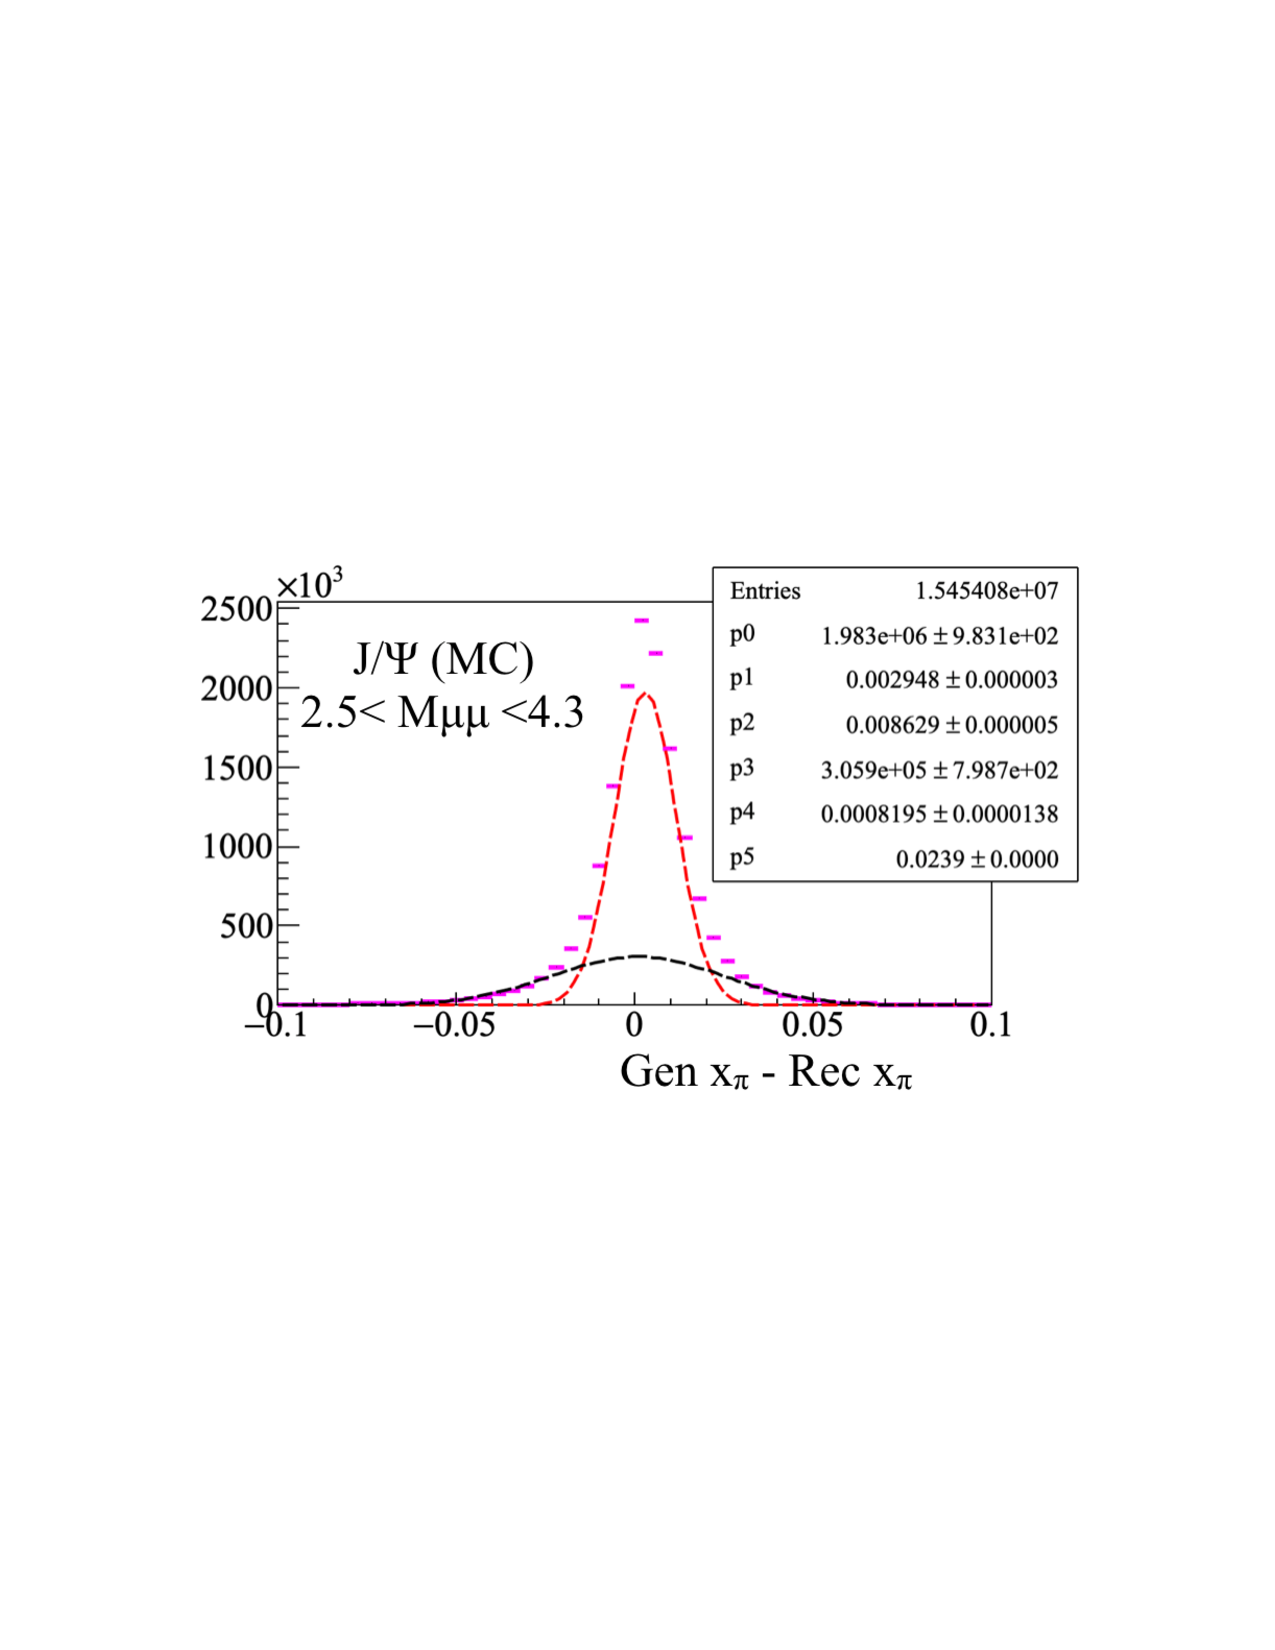
\includegraphics[width=0.6\textwidth, trim=3cm 9cm 3cm 9cm,clip]{JPsiXPiRes}
  \caption{The distribution of generated $x_N$ minus reconstructed $x_N$.  The
    leading Gaussian width (red) is used to determine the resolution.}
  \label{fig::JPsiXPiRes}
\end{figure}

\begin{table}[h!t]
  \centering
  \begin{tabular}{ |c|c|c| }
    \hline \textbf{Variable}& \textbf{RMS}& \textbf{Leading Gaussian $\sigma$}
    \\ \hline \hline
    
    $x_N$& 0.01& 0.006 \\ \hline

    $x_\pi$& 0.0157& 0.009 \\ \hline

    $x_F$& 0.016& 0.011 \\ \hline

    $q_T$& 0.143& 0.022 \\ \hline
  \end{tabular}
  \caption{COMPASS spectrometer resolutions in the intermediate mass range
    2.5-4.3{\gvcw}}
  \label{tab::JPsiRes}
\end{table}

\begin{table}[h!t]
  \begin{adjustwidth}{-1.4cm}{}
  \centering
  \begin{tabular}{ |c|c|c|c|c|c| }
    \hline \textbf{Variable}& \textbf{Lowest limit}& \textbf{Upper limit bin
      1}& \textbf{Upper limit bin 2}& \textbf{Upper limit bin 3}&
    \textbf{Upper limit bin 4}\\ \hline
    
    $x_N$& 0.0& 0.062& 0.083& 0.11& 1.0\\ \hline
    
    $x_{\pi}$& 0.0& 0.21& 0.28& 0.38& 1.0\\ \hline
    
    $x_F$& -1.0& 0.10& 0.20& 0.32& 1.0\\ \hline
    
    $q_T$ (GeV/c)& 0.4& 0.72& 1.04& 1.47& 5.0\\ \hline
    
    $M_{\mu\mu}$ (GeV/c$^2$)& 2.87& 3.03& 3.13& 3.22& 3.38 \\ \hline
    
  \end{tabular}
  \caption{The {\jp} analysis bin limits for the four analysis bins}
  \label{tab::JPsi_binning}
  \end{adjustwidth}
\end{table}

The distributions for the binning variables are shown in
Fig.~\ref{fig::JPsi_Kinematics}.  This analysis is performed in the valence
region for both the beam pion and target proton as the average $x_\pi$ is about
0.09 and the average $x_N$ is about 0.3.  This means the dominant contribution
to {\jp} production is from quark-quark interactions.  The average $q_T$ value
is below the minimum mass range of 2.87~{\gvcw} for this analysis and therefore
the interpretation of this analysis assumes the TMD regime is valid.

\begin{figure}[h!t]
  \centering 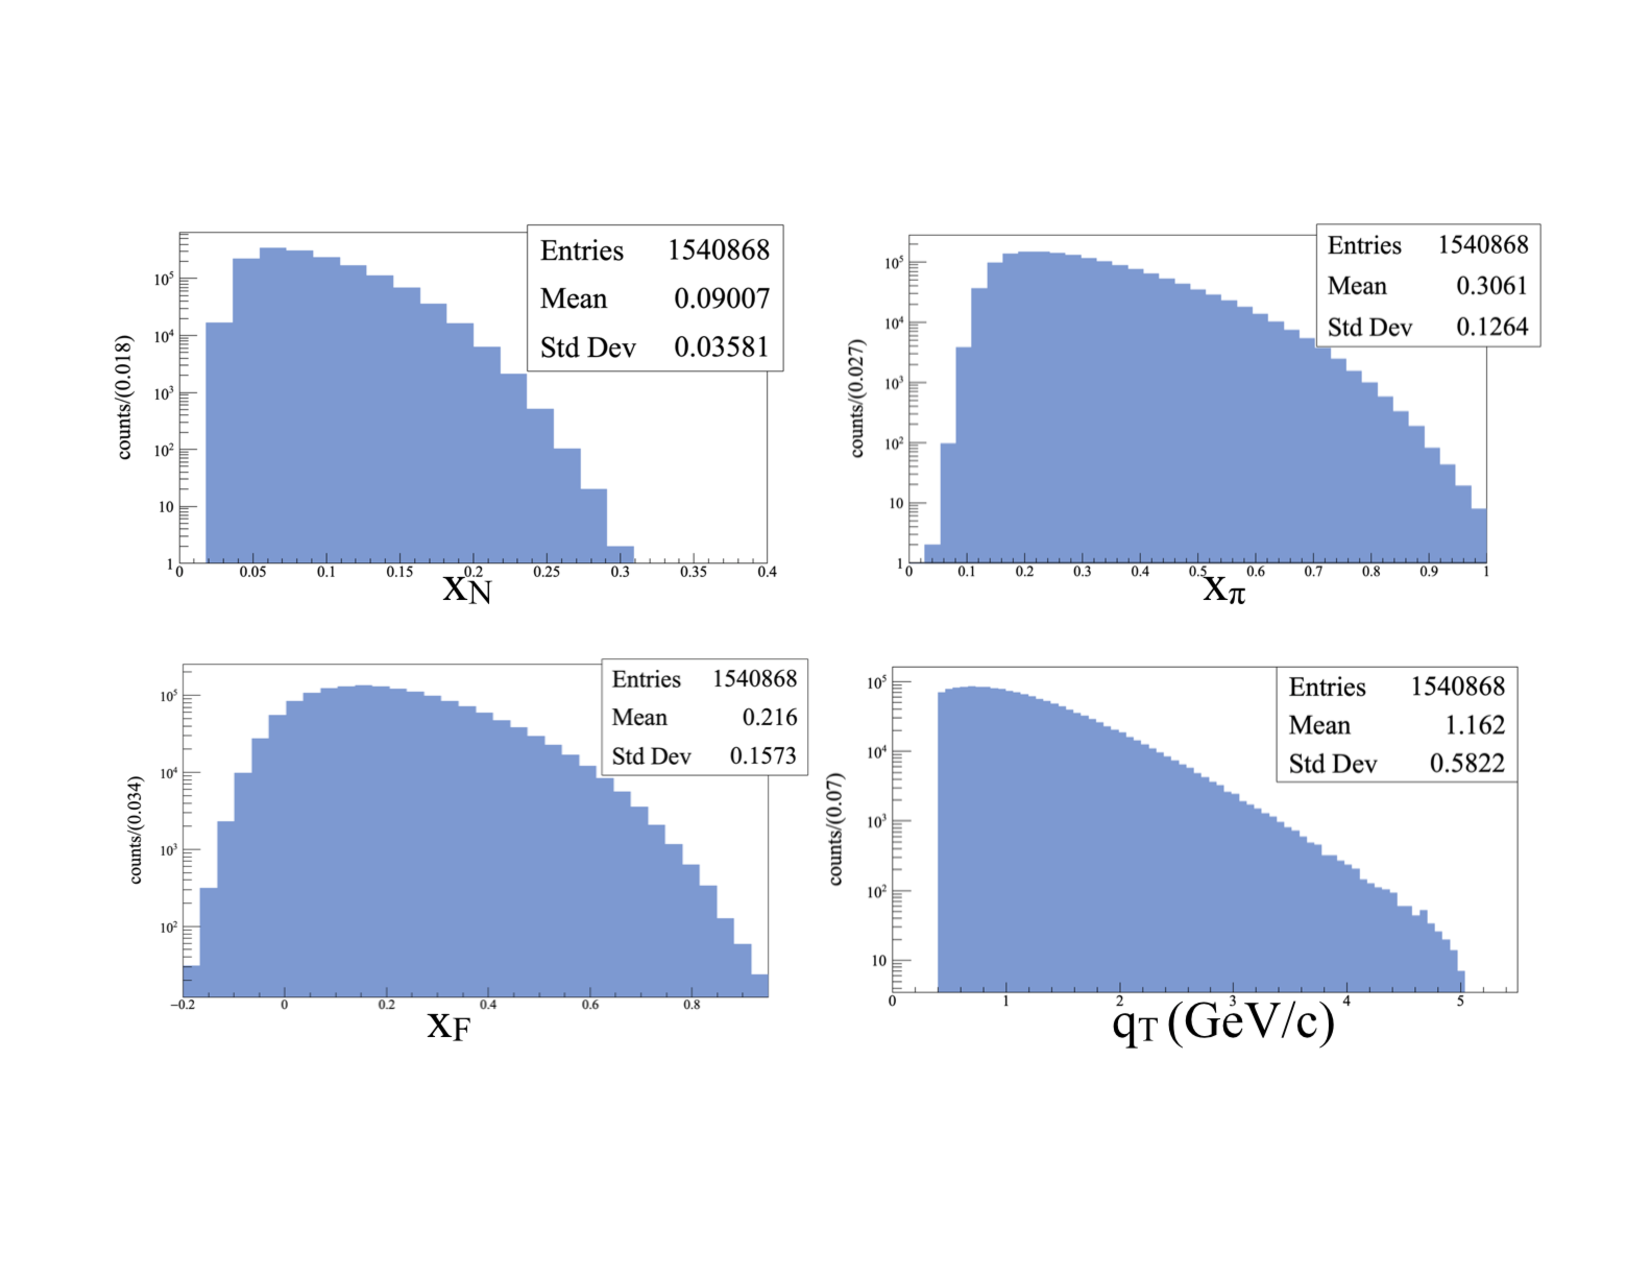
\includegraphics[width=0.95\textwidth,trim=1cm 3.5cm 1cm
    3.5cm,clip]{JPsi_Kinematics}
  \caption{The binning variable distributions. The longitudinal momentum
    fractions $x_N$ (top left) and $x_\pi$ (top right) and the $x_F$ (bottom
    left) and the virtual photon transverse momentum $q_T$ (bottom right).
    These distributions are plotted from in the mass range 2.87-3.38~{\gvcw}.}
  \label{fig::JPsi_Kinematics}
\end{figure}


\subsection{Asymmetry Extraction}
The asymmetry extraction method used is the two-target geometric mean.  This
asymmetry method is described in detail in
Secs~\ref{sec::leftrightasym}-~\ref{sec::TwoTargGeoMean}.  The asymmetry is
again defined as

\begin{equation}
  \label{equ::AN4TargGeomeanJPsi}
  A_{lr,2Targ} =
  \frac{1}{|S_T|}
  \frac{ \sqrt[4]{ N_{1,l}^\uparrow N_{1, l}^\downarrow
      N_{2,l}^\uparrow N_{2, l}^\downarrow }
    - \sqrt[4]{ N_{1,r}^\uparrow N_{1,r}^\downarrow
      N_{2,r}^\uparrow N_{2,r}^\downarrow }
  }{
    \sqrt[4]{ N_{1,l}^\uparrow N_{1, l}^\downarrow
      N_{2,l}^\uparrow N_{2, l}^\downarrow }
    + \sqrt[4]{ N_{1,r}^\uparrow N_{1,r}^\downarrow
      N_{2,r}^\uparrow N_{2,r}^\downarrow } },
\end{equation}
\noindent
where $N$ represents the counts, $l(r)$ denotes left(right), 1(2) denotes the
target cell and $\uparrow(\downarrow)$ denotes the transverse polarization
direction.  The definitions of left and right are defined relative to the target
spin as
\begin{equation}
  \begin{aligned}
    \text{Left} &: \hat{q}_T \cdot (\hat{S}_T \times \hat{P}_{\pi}) > 0 \\
    \text{Right} &: \hat{q}_T \cdot (\hat{S}_T \times \hat{P}_{\pi}) < 0, 
  \end{aligned}
\end{equation}
\noindent
where $\hat{q}_T$, $\hat{S}_T$ and $\hat{P}_{\pi}$ are unit vectors in the
target reference frame for the virtual photon transverse momentum, the target
spin and the beam pion momentum respectively.  The advantage of this asymmetry
method is that the acceptance from the upstream and downstream target cells
cancel as was shown in Eq.~\ref{equ::AN2targAcceptCancel}.  The statistical
uncertainty for this asymmetry method can be written as

\begin{equation}
  \delta A_{lr,2Targ} = \frac{1}{|S_T|}
  \frac{LR}{\Big( L+R \Big)^2}
  \sqrt{
    \sum_{c,p}
    \Big(
    \frac{1}{N_{c,l}^{p}}
    + \frac{1}{N_{c,r}^p}
    \Big)
  } \quad,
\end{equation}
where $L =\sqrt[4]{N_{1,l}^\uparrow N_{1,l}^\downarrow N_{2,l}^\uparrow
  N_{2,l}^\downarrow}$ and $R =\sqrt[4]{N_{1,r}^\uparrow N_{1,r}^\downarrow
  N_{2,r}^\uparrow N_{2,r}^\downarrow}$.  In the approximate case of equal
statistical populations in each left-right direction and each target cell, the
statistical uncertainty for the two-target geometric mean reduces to
$\frac{1}{|S_T|}\frac{1}{\sqrt{N}}$, where $N$ is the sum of all counts.

\subsection{Systematic Studies}
Similar tests as were performed for the high mass left-right asymmetry to
determine the systematic error are also performed for the intermediate mass
left-right asymmetry.  For the full details on the previous tests see
Sec~\ref{sec::systematics}.  This section will give the results for systematic
errors in the intermediate mass range and describe in detail the tests specific
to this analysis.  The overall systematic errors are determined by adding all
non-zero systematic uncertainties in quadrature.  The impact from each source of
systematic error is summarized in Table.~\ref{tab::sysErrorJPsi}.

\subsubsection{Period Compatibility (Time Dependence)}
It is expected that the asymmetry calculation will vary in time due to
statistical fluctuations.  Fig.~\ref{fig::JPsi_AlrPeriod} shows the left-right
asymmetry calculated for each period in time and Fig.~\ref{fig::JPsi_AlrXn}
shows the left-right asymmetry time fluctuations for each bin in $x_N$.  To
quantify if the time fluctuations are greater than what is expected from random
statistical fluctuations, the pull distribution is checked for a larger width
than one or a non-zero mean.  More details on the pull distribution are given in
Sec~\ref{sec::sysPulls}.

\begin{figure}[h!t]
  \centering 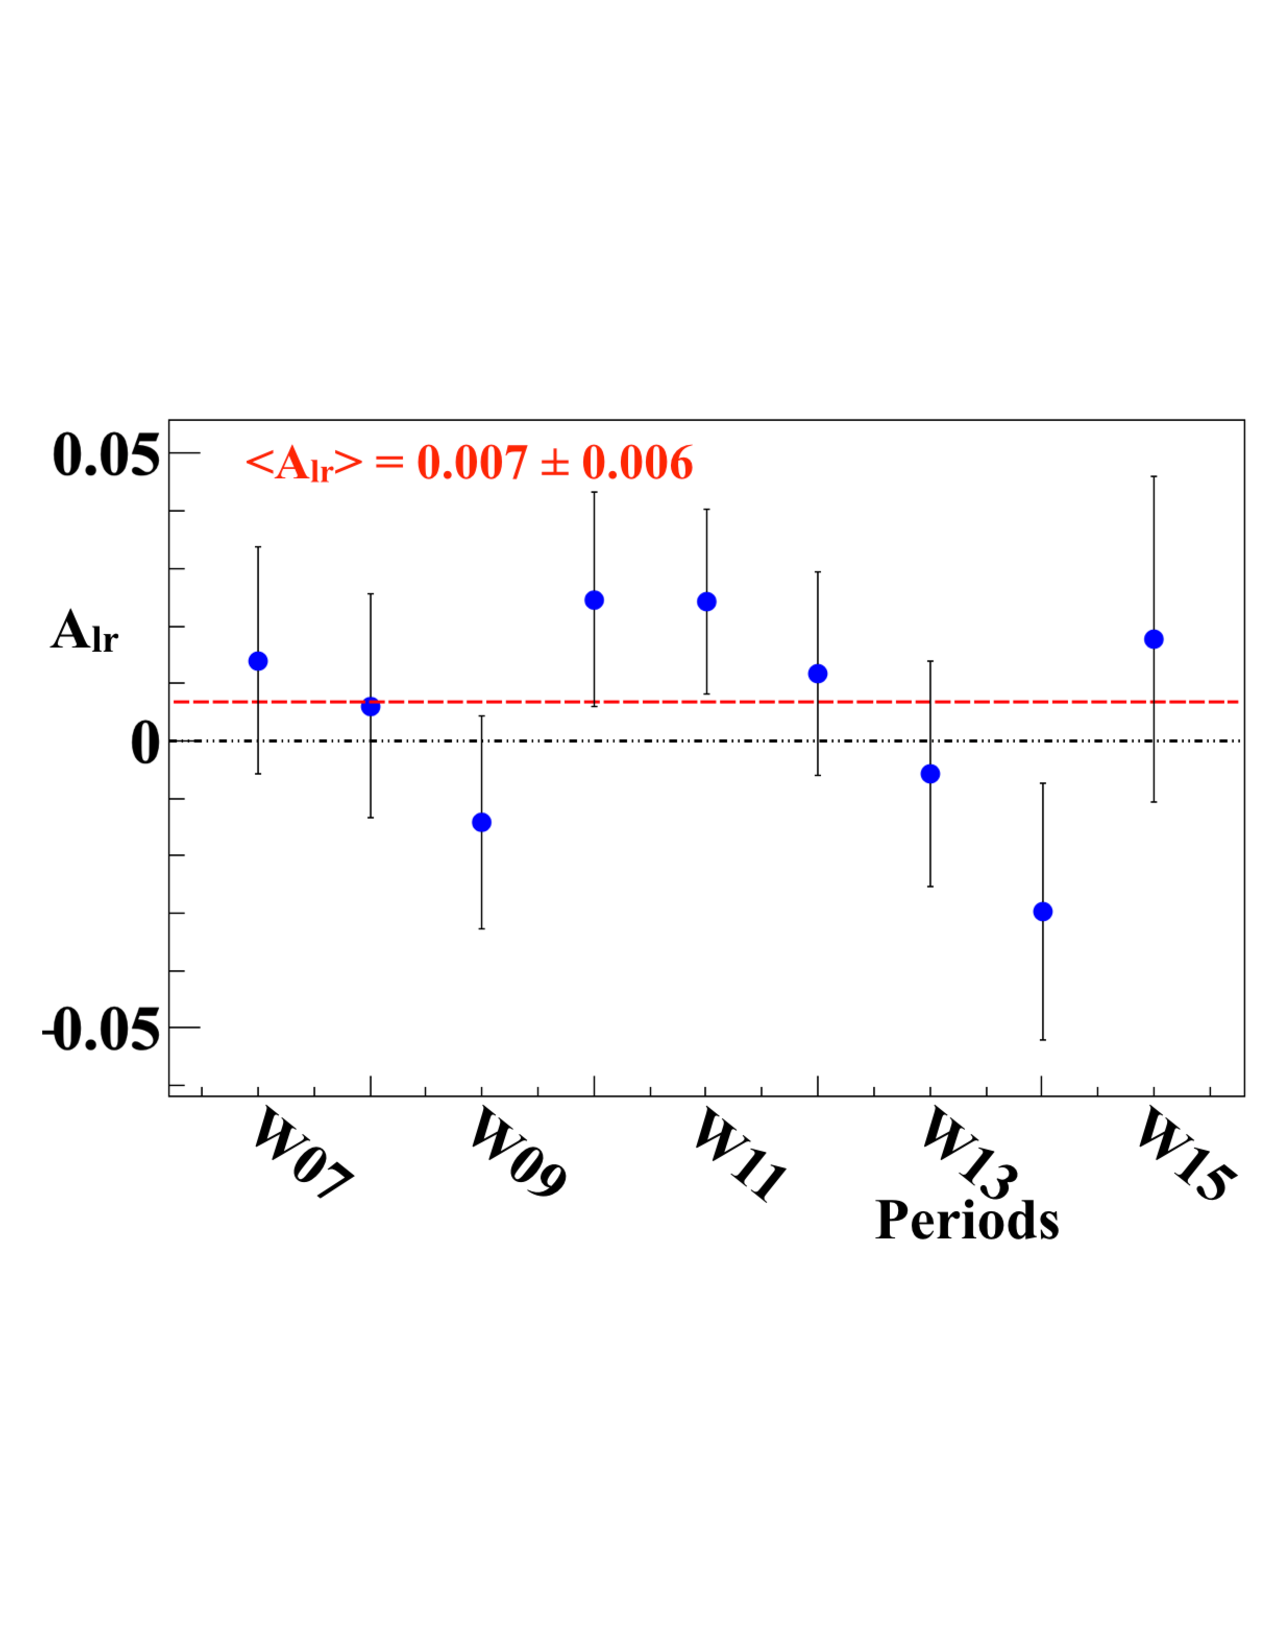
\includegraphics[width=0.65\textwidth,trim=0.5cm 6cm 0.5cm
    6cm,clip]{JPsi_AlrPeriod}
  \caption{The left-right asymmetry in the {\jp} mass region as a function of
    time.  The red line is a constant fit and therefore shows the weighted
    averaged of the periods.}
  \label{fig::JPsi_AlrPeriod}
\end{figure}

\begin{figure}[h!t]
  \centering
  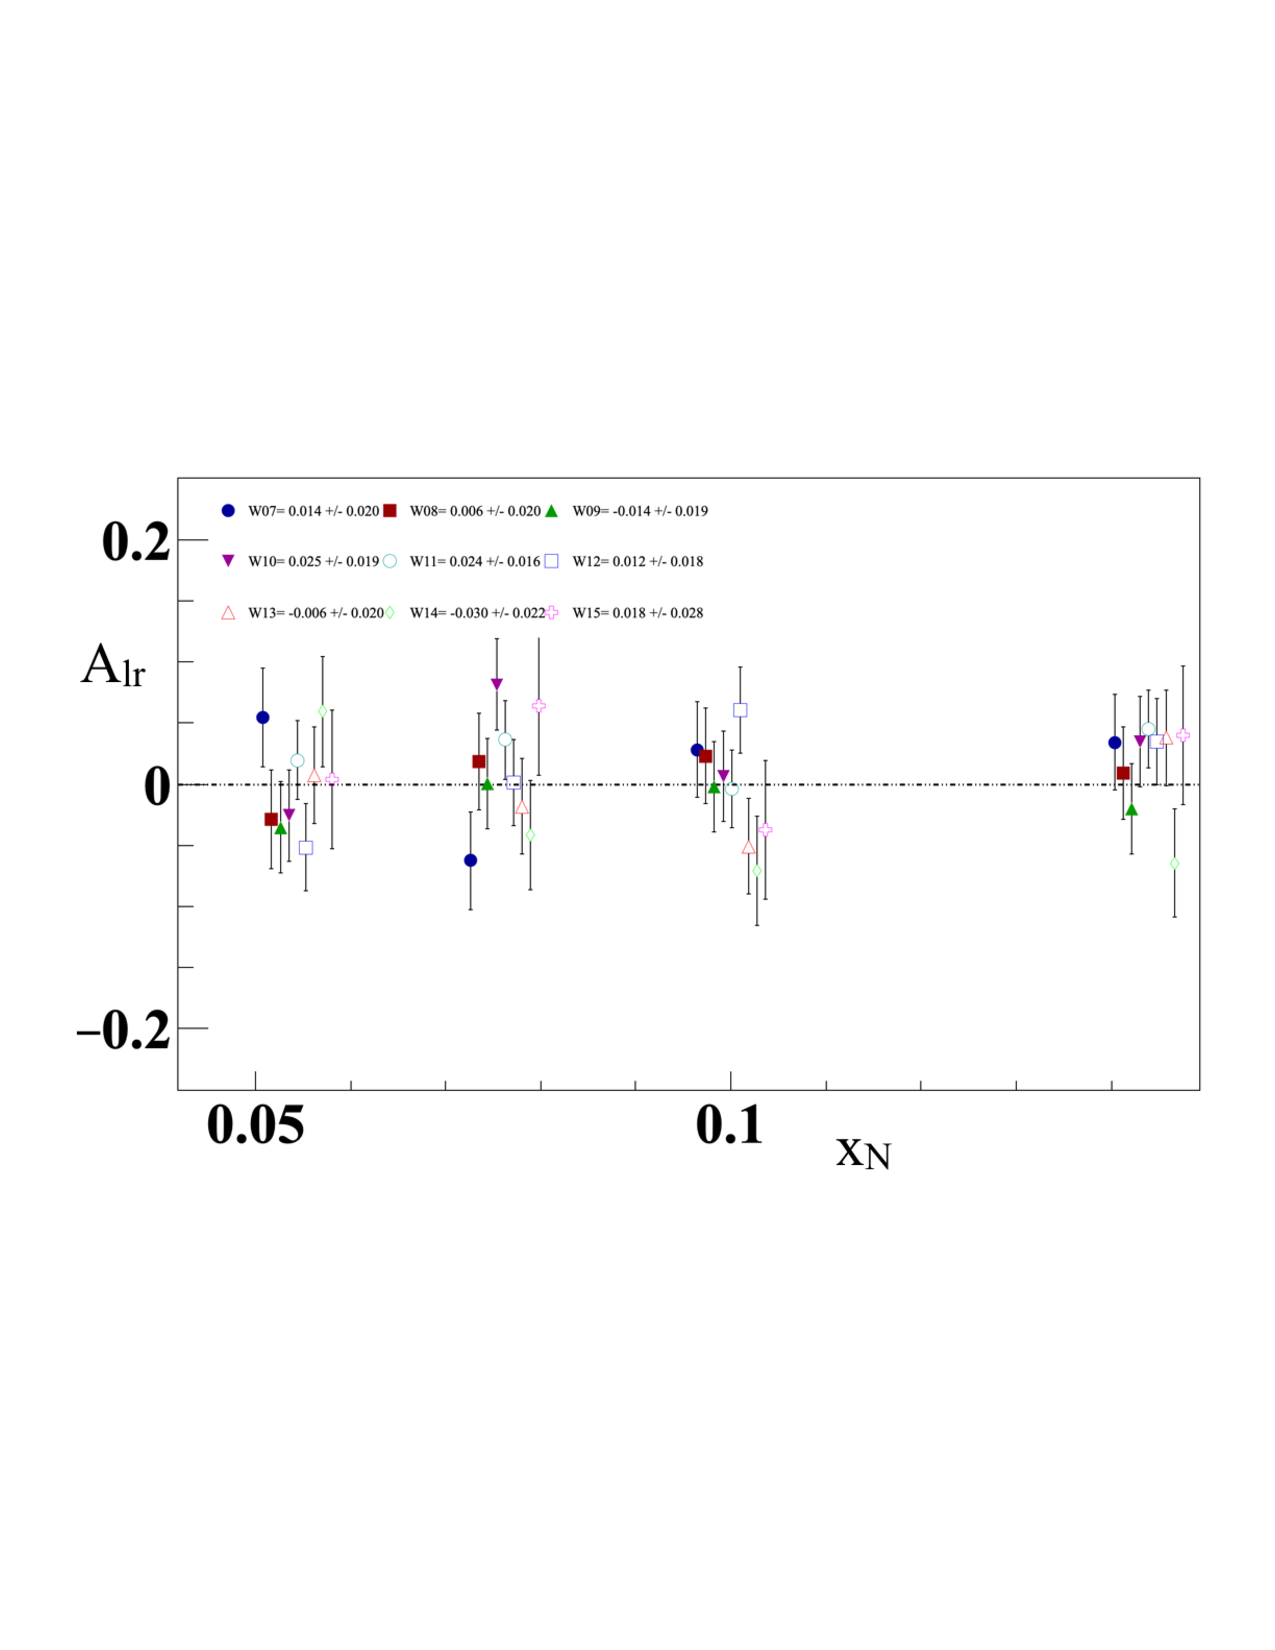
\includegraphics[width=0.65\textwidth,trim=1cm 8cm 1cm 8cm,clip]{JPsi_AlrXn}
  \caption{The left-right asymmetry time fluctuations in each bin of $x_N$.}
  \label{fig::JPsi_AlrXn}
\end{figure}

The pull value is defined as
\begin{equation}
  \label{eq::pullJPsi}
  \Delta\mathrm{A}_i =
  \frac{
    \mathrm{A}_i - \langle \mathrm{A} \rangle
  }{
    \sqrt{
      \sigma^2_{\mathrm{A}_i} - \sigma^2_{\langle \mathrm{A} \rangle}
    }
  },
\end{equation}
\noindent
where $\langle \mathrm{A} \rangle$ is the average asymmetry amplitude for the
data set.  The pull distribution is formed for each kinematic variable in
Fig.~\ref{fig::JPsi_Pulls}.  For this analysis there are therefore 4 (number of
bins) x 9 (number of periods) = 36 entries per pull distribution.  The
systematic error from period incompatibility is determined as

\begin{equation}
  \label{equ::sysErrorPullJPsi}
  \frac{\sigma_{systematic}}{\sigma_{statistical}} =
  \sqrt{|\sigma^2_{pull} - 1|} + \frac{\mu_{pull}}{2},
\end{equation}
\noindent
where in this analysis the $\sigma_{pull}^2$ and $\mu_{pull}$ are determined as
a weighted average of the mean and variance respectively from the pull
distribution for each kinematic variable including the parameters from the
integrated pull distribution.  The fit values from each pull distribution give
somewhat different estimates due to the errors associated with the fit.  This is
the reason the weighted average is performed to give the best estimate for the
pull mean and standard deviation and therefore the most accurate systematic
error calculation.  The systematic error due to time incompatibility is
determined to be 16\% of the statistical error.

\begin{figure}[h!t]
  \centering 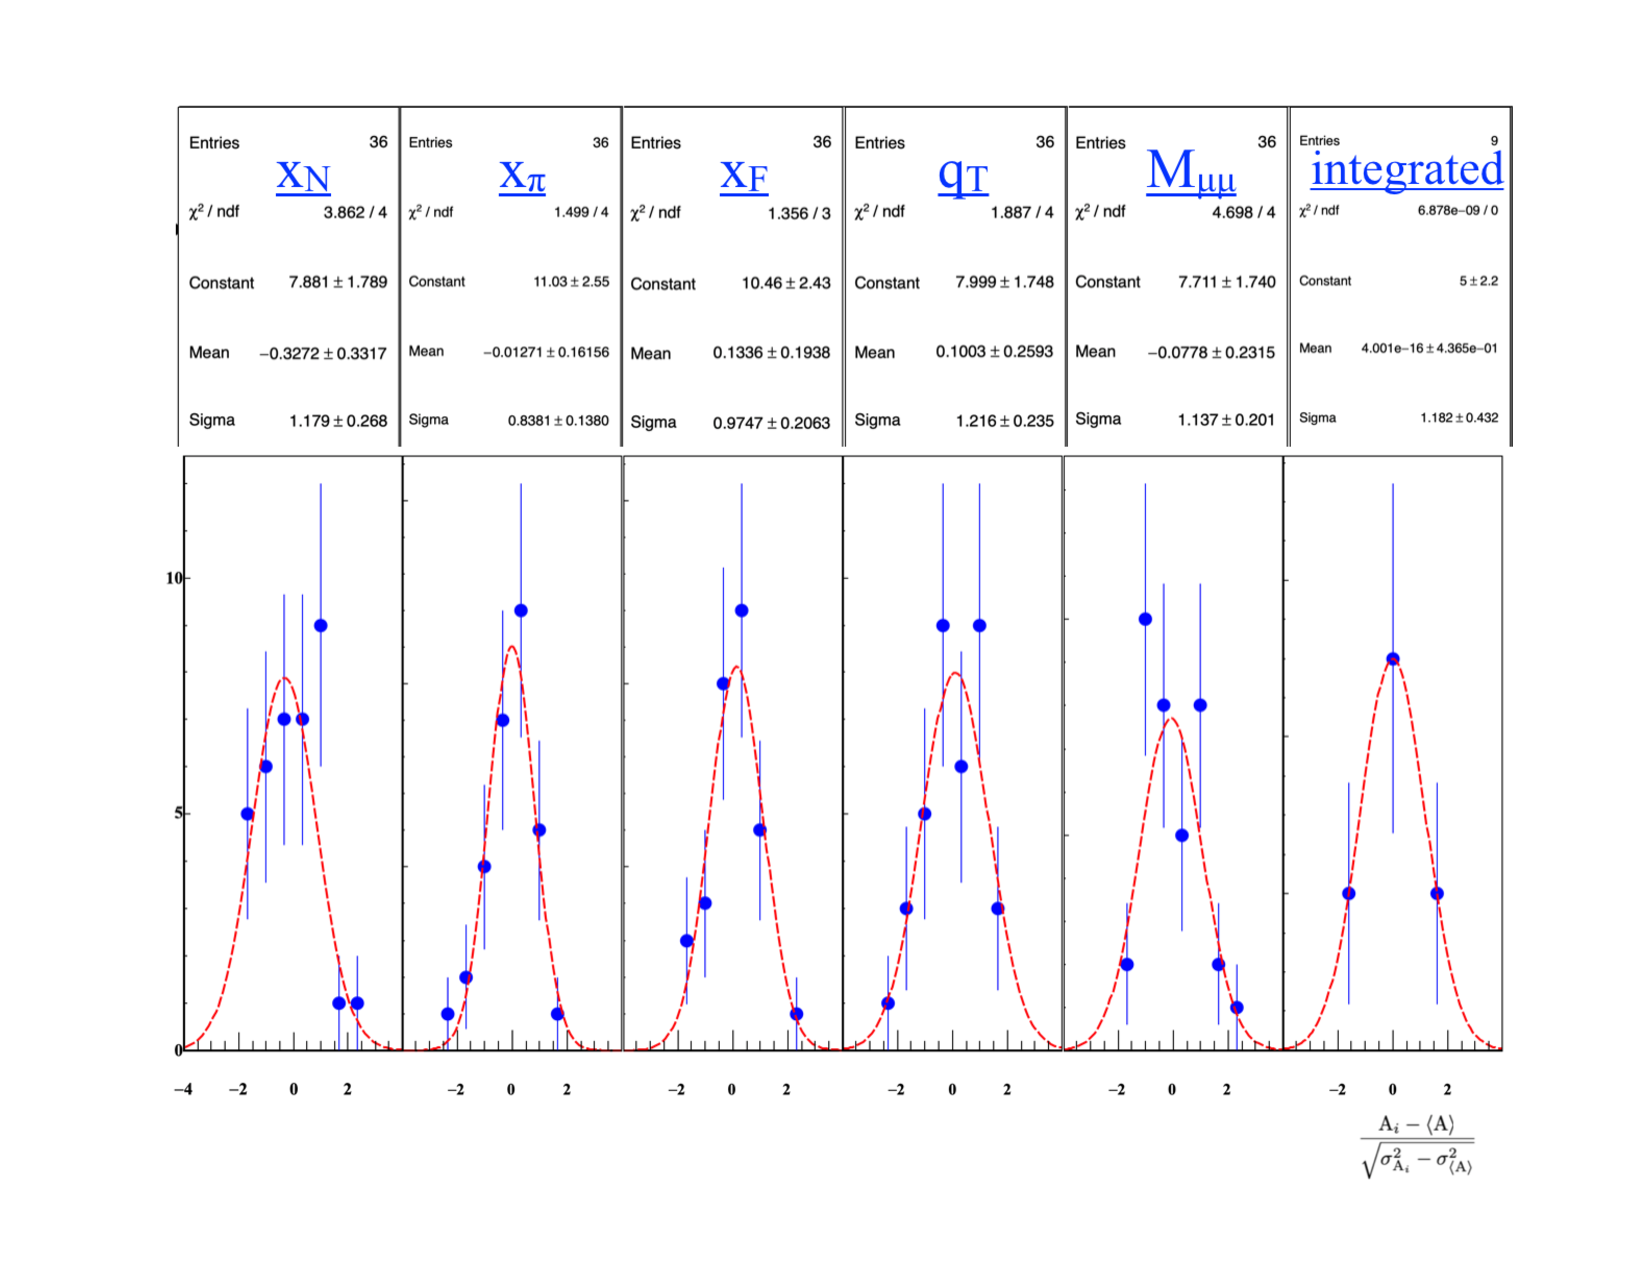
\includegraphics[width=\textwidth,trim=2.2cm 1.7cm 2.2cm
    1.7cm,clip]{JPsi_Pulls}
  \caption{The uncorrelated pull distributions for each of the kinematical
    variables and a pull distribution from the integrated asymmetry from each
    time period.}
  \label{fig::JPsi_Pulls}
\end{figure}


\subsubsection{Left/Right Event Migration}
The left-right event migration systematic error is calculated the same as in
Sec~\ref{sec::syslrEventMigration}.  The Monte-Carlo data used to determine the
left-right event migration is described in Table~\ref{tab::MCproduction}.  The
effect of misidentified events as left when the event should be counted as a
right event and vise-versa, dilutes the left-right asymmetry.  It is as if
there is an additional unpolarized contribution that dilutes the event sample.

The systematic error for left-right migration is derived in
Appendix~\ref{app::sysLRmiss} as

\begin{equation}
  \delta A_{lr,systematic} = \gamma *A_{lr} + \gamma *\delta A_{lr},
\end{equation}
\noindent
where $\gamma$ is the fraction of misidentified left and right events.  

As is clearly visible in Fig.~\ref{fig::JPsilrMigration}, there is a band of
higher misidentification rate at the border between left and right.  For the
{\jp} mass region only about 3\% of events were misidentified resulting in a
systematic error of 4.4\% of the statistical error.

\begin{figure}[h!t]
  \centering 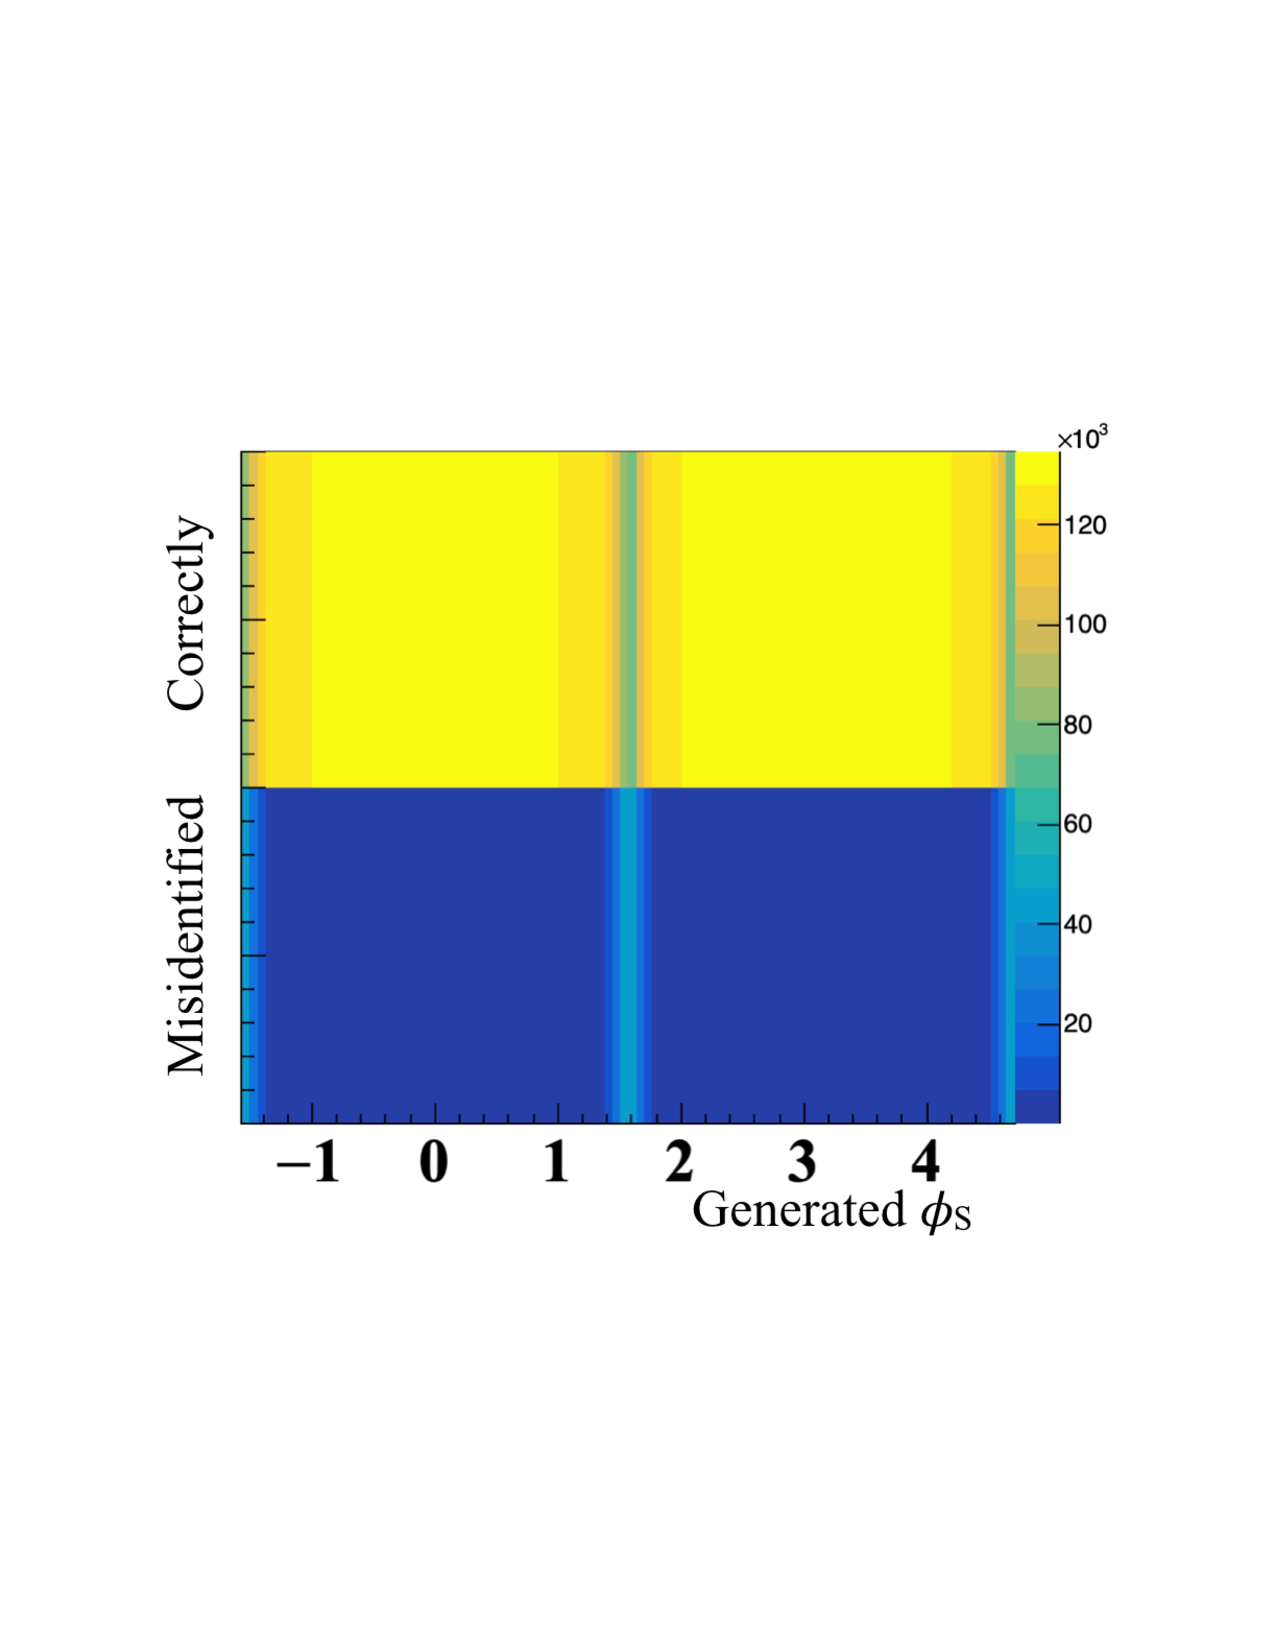
\includegraphics[width=0.4\textwidth,trim=2cm 7cm 2cm
    7cm,clip]{JPsilrMigration}
  \caption{The left-right migration as a function of the generated $\phi_S$
    angle in the mass range 2.87-3.38.}
  \label{fig::JPsilrMigration}
\end{figure}

\subsubsection{J/$\Psi$ Purity}

The systematic error due to a {\jp} purity less than unity was discussed in
Sec~\ref{sec::jpMassRange}.  The invariant mass range was chosen specifically
such that the {\jp} purity is 90\% or higher to reduce the systematic error
associated with impurities.  The systematic error is derived in
Appendix~\ref{app::sysEventContam} as

\begin{equation}
  \frac{\sigma_{systematic}}{\sigma_{statistical}} = \frac{(1-p)}{p}.
\end{equation}
\noindent
Table~\ref{tab::JPsiPurity} summarized the impurity as a function of the
analysis mass range and the impurity in this analysis mass range is 91.3\%.
This corresponds to a systematic error of 9.5\% of the statistical error.

\subsubsection{False Asymmetries}
\subsubsection{Acceptance From False Asymmetries}
The acceptance fluctuations are determined from the false asymmetry defined as
\begin{equation}
  A_{lr,False} = 
    \frac{1}{|S_T|}
    \frac{
      \sqrt[4]{
        N_{1,r}^\uparrow N_{1, l}^\downarrow
        N_{2,l}^\uparrow N_{2, r}^\downarrow
      } 
      -\sqrt[4]{
        N_{1,l}^\uparrow N_{1, r}^\downarrow
        N_{2,r}^\uparrow N_{2, l}^\downarrow
      }
    }{
      \sqrt[4]{
        N_{1,r}^\uparrow N_{1, l}^\downarrow
        N_{2,l}^\uparrow N_{2, r}^\downarrow
      } +
      \sqrt[4]{
        N_{1,l}^\uparrow N_{1, r}^\downarrow
        N_{2,r}^\uparrow N_{2, l}^\downarrow
      }
    } 
    = \frac{1}{|S_T|}
    \frac{
      \alpha_{2Targ} - 1     
    }{
      \alpha_{2Targ} + 1
    }.
    \label{equ::falseAccJPsi}
\end{equation}
\noindent
More details for acceptance fluctuations are discussed in
Sec.~\ref{sec::GeoMean} and Sec.~\ref{sec::TwoTargGeoMean}.  The kinematic
dependencies of the acceptance ratio, $\alpha_{2Targ}$, are shown in
Fig.~\ref{fig::alphaJPsi}.  As Fig.~\ref{fig::alphaJPsi} shows the acceptance is
only slightly greater than unity even though it can be above 1 by more than a
sigma.  The systematic error associated with acceptance fluctuations is defined
as

\begin{equation}
  \delta A_{lr,systematic} =
  \frac{1}{|S_T|}
  \Big(\frac{|\alpha_{2Targ}-1|}{2}
  + \delta_{\frac{|\alpha_{2Targ}-1|}{2}} \Big),
\end{equation}

\noindent
where this expression is derived in Appendix~\ref{app::sysAcc}.  The normalized
kinematic dependence of the systematic error to the statistical error are shown
in Fig.~\ref{fig::accSysStatJPsi}.  The average systematic error due to
acceptance is 23\% of the statistical error.

\begin{figure}[h!t]
  \begin{center}
    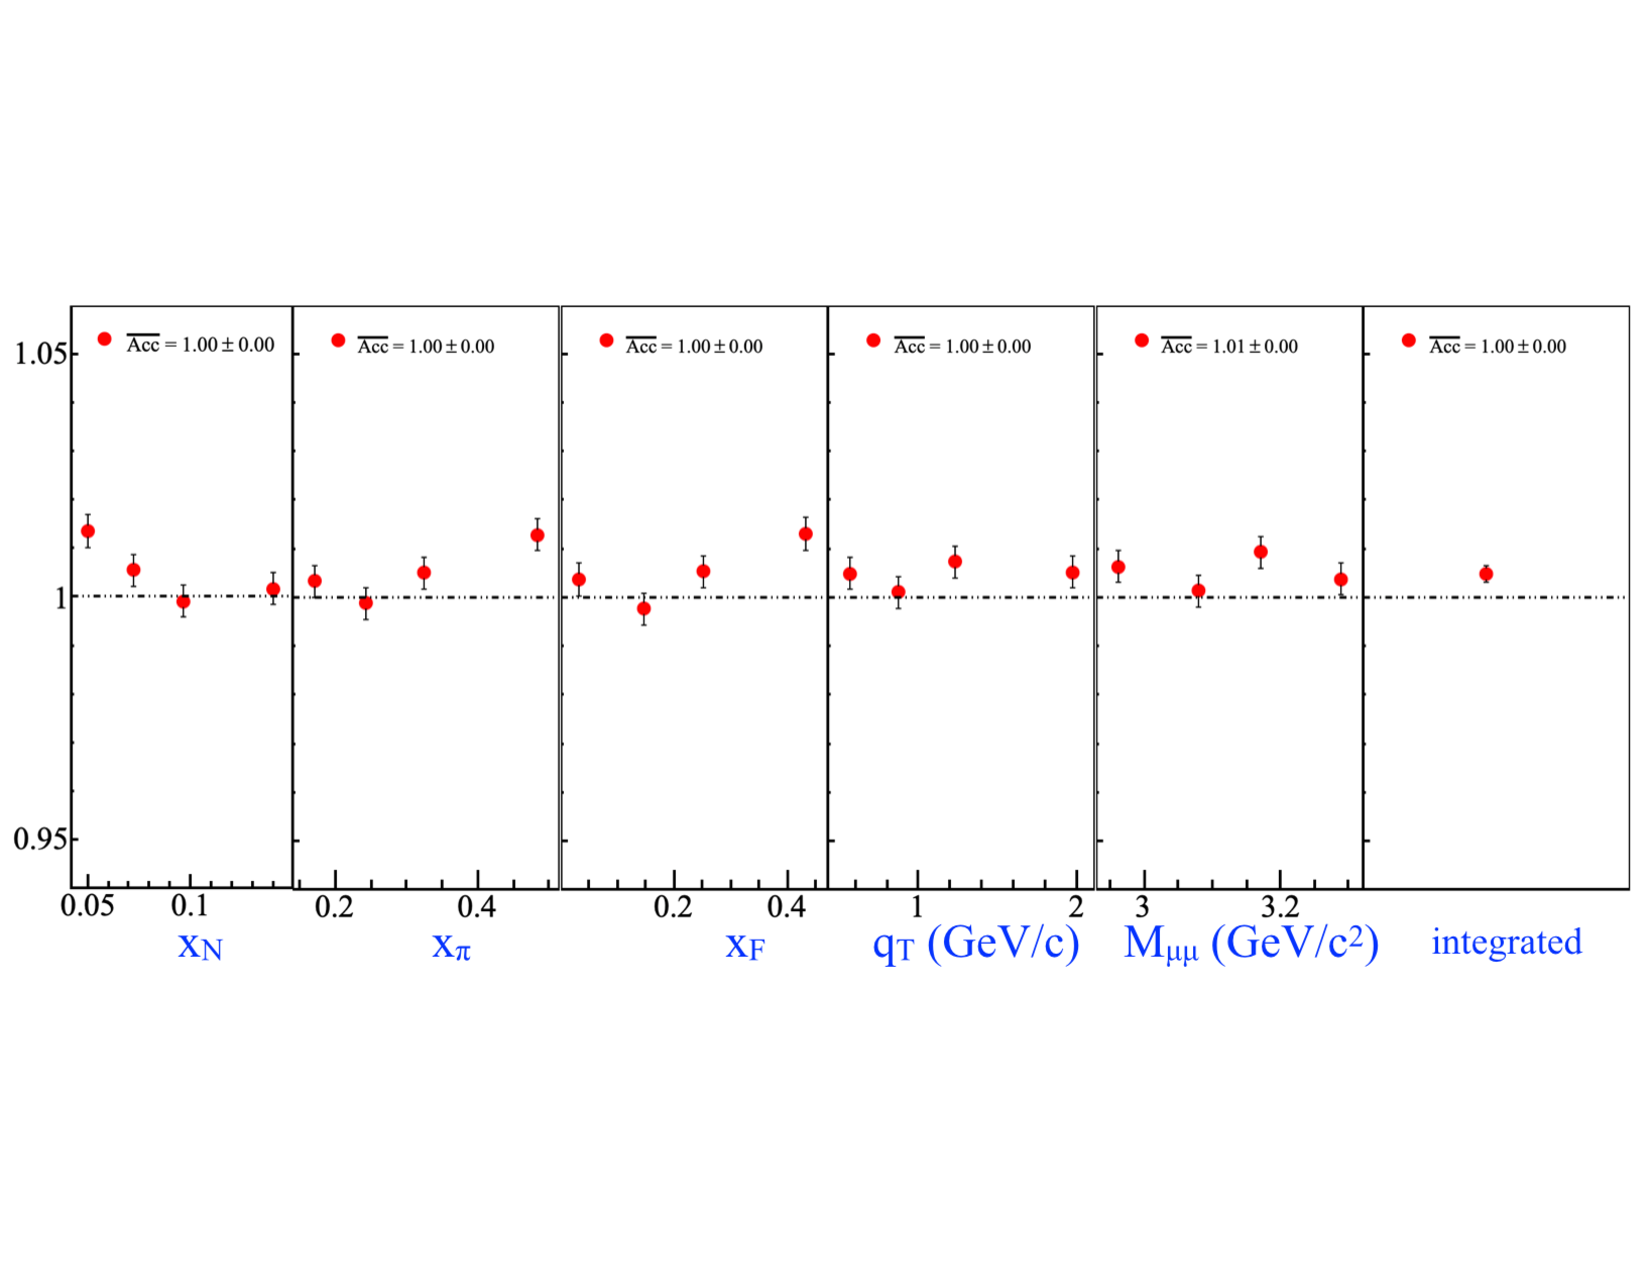
\includegraphics[width=\textwidth, trim=0cm 5cm 0cm 5cm,
      clip]{alphaJPsi}
    \caption{Acceptance fluctuations in each bin of the kinematic variables.}
    \label{fig::alphaJPsi}
  \end{center}
\end{figure}

\begin{figure}[h!t]
  \begin{center}
    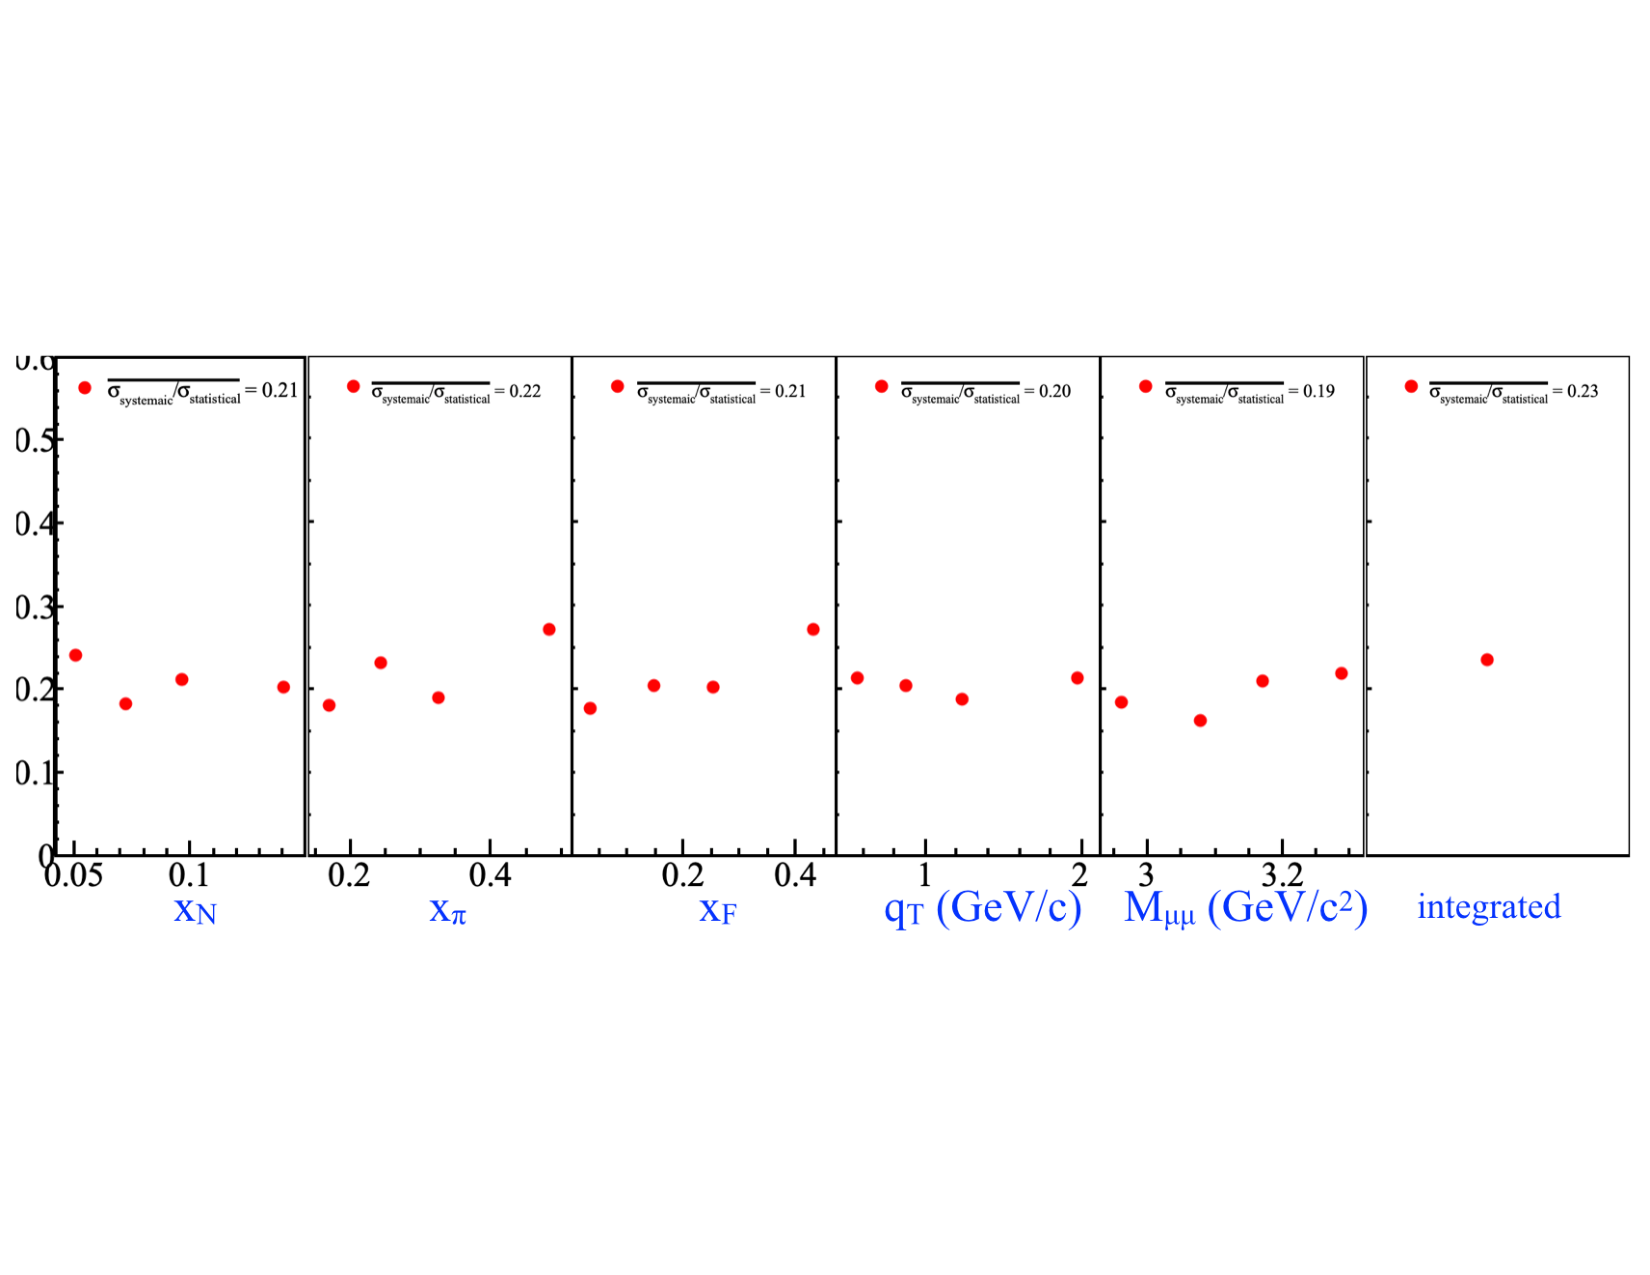
\includegraphics[width=\textwidth, trim=0cm 5cm 0cm 5cm,
      clip]{accSysStatJPsi}
    \caption{Systematic error divided by statistical error due to acceptance}
    \label{fig::accSysStatJPsi}
  \end{center}
\end{figure}

\subsubsection{Further False Asymmetry Effects}
Additional false asymmetries are analyzed to account for systematic errors which
were not addressed directly.  The false asymmetries are constructed in such a
way that the cross-section and luminosity cancel out in the numerator and the
denominator.  Therefore these false asymmetries can only change in time due to
acceptance effects or for some unknown reason.  The false asymmetries
constructed to study the intermediate mass analysis are described in the
following enumerated list.

\begin{enumerate}
  \label{tab::additionalFAJPsi}

\item The false asymmetry used to determine the acceptance fluctuations,
  Eq.~\ref{equ::falseAccJPsi}, is checked for compatibility and the
  uncorrelated pulls are shown in Fig.~\ref{fig::fa2TargPullsJPsi} along with
  the corresponding fit parameters and errors.

  \begin{figure}[h!t]
    \centering 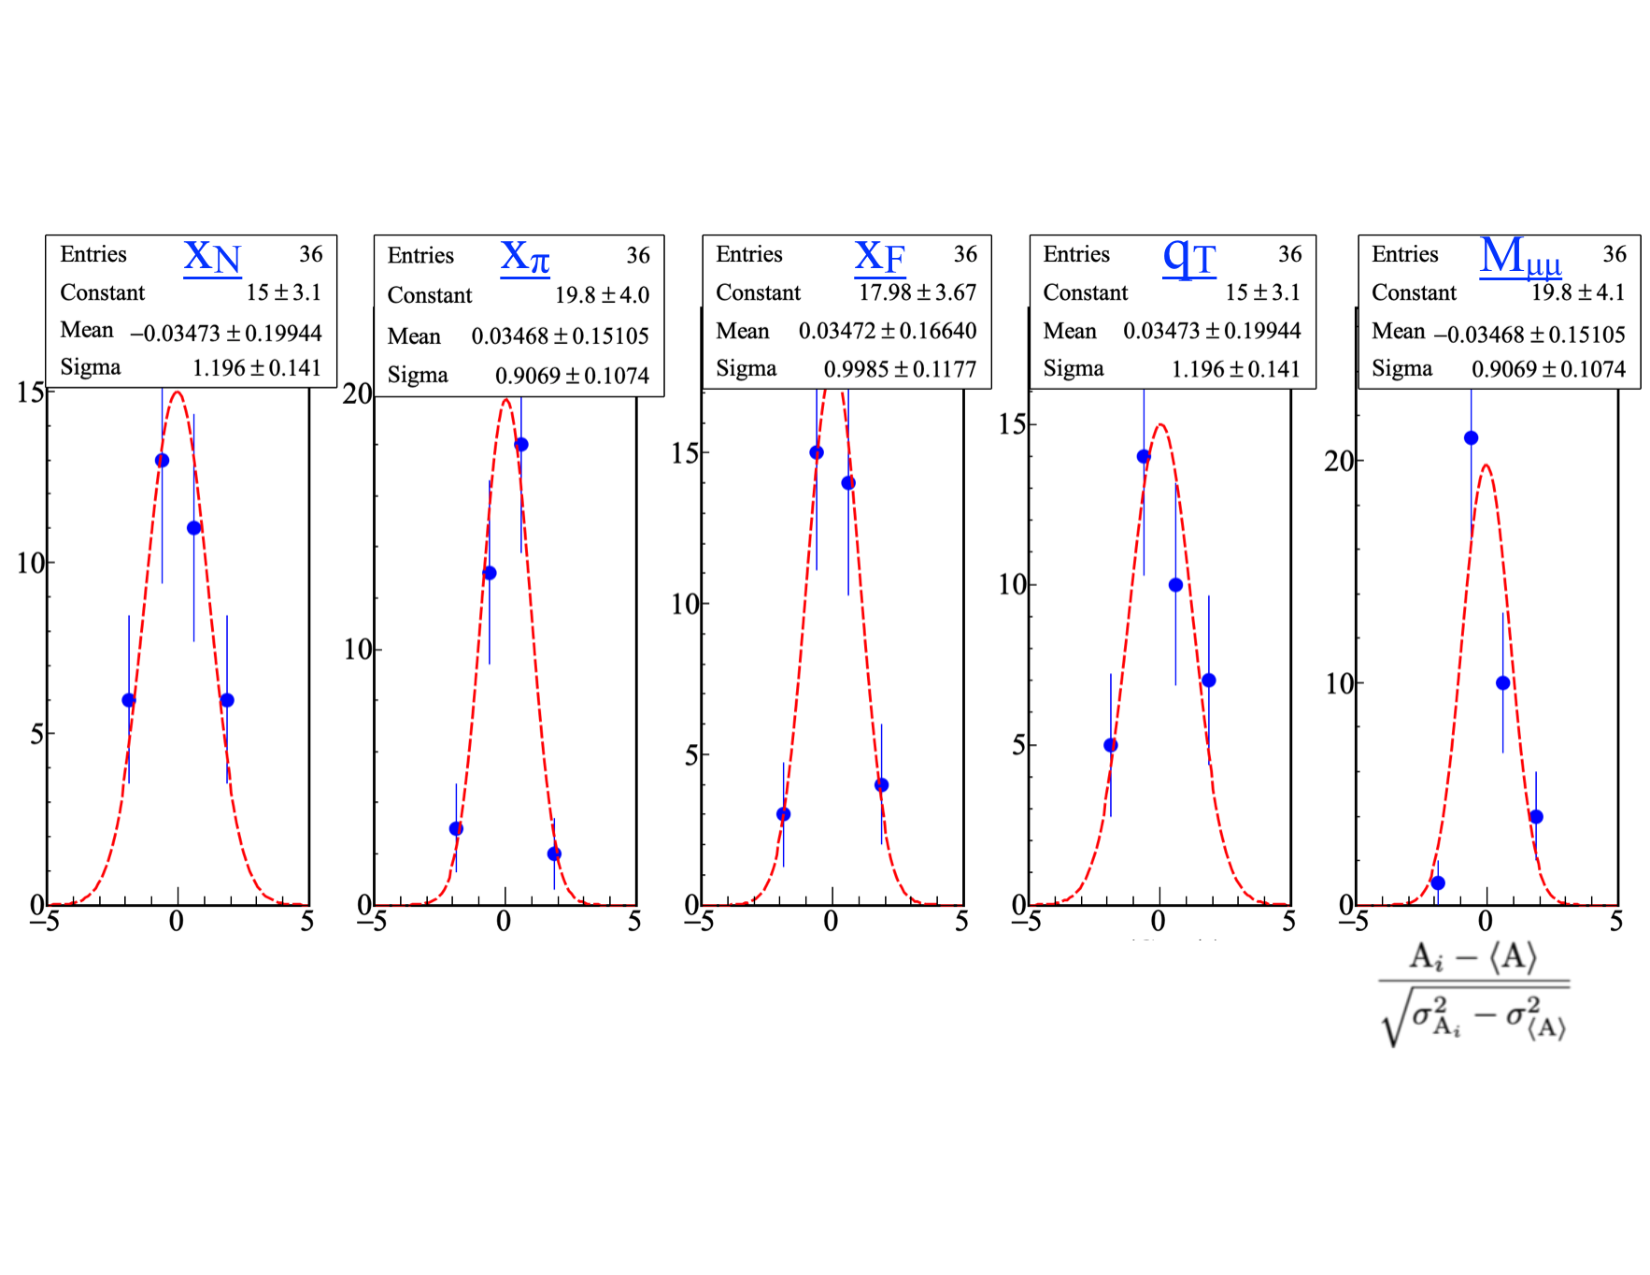
\includegraphics[width=\textwidth, trim=0cm 3cm 0cm 3cm,
      clip]{fa2TargPullsJPsi}
    \caption{Pull distribution for a nearly acceptance free two-target false
      geometric mean asymmetry}
    \label{fig::fa2TargPullsJPsi}
  \end{figure}

  \item A false asymmetries using only the information from the upstream or the
  downstream target cell defined as

  \begin{equation}
    \label{equ::falseANgeomeanJPsi}
    A_{lr, FA} =
    \frac{1}{|S_T|}
    \frac{\sqrt{N_l^\uparrow N_r^\downarrow}
      - \sqrt{N_r^\uparrow N_l^\downarrow}
    }{
      \sqrt{N_l^\uparrow N_r^\downarrow}
      + \sqrt{N_r^\uparrow N_l^\downarrow}
    }.
  \end{equation}
  The pulls for the upstream target cell are shown in
  Fig.~\ref{fig::faPullsUpSJPsi} and the pulls for the downstream target cell
  are shown in Fig.~\ref{fig::faPullsDownSJPsi}.

  \begin{figure}[h!t]
  \centering 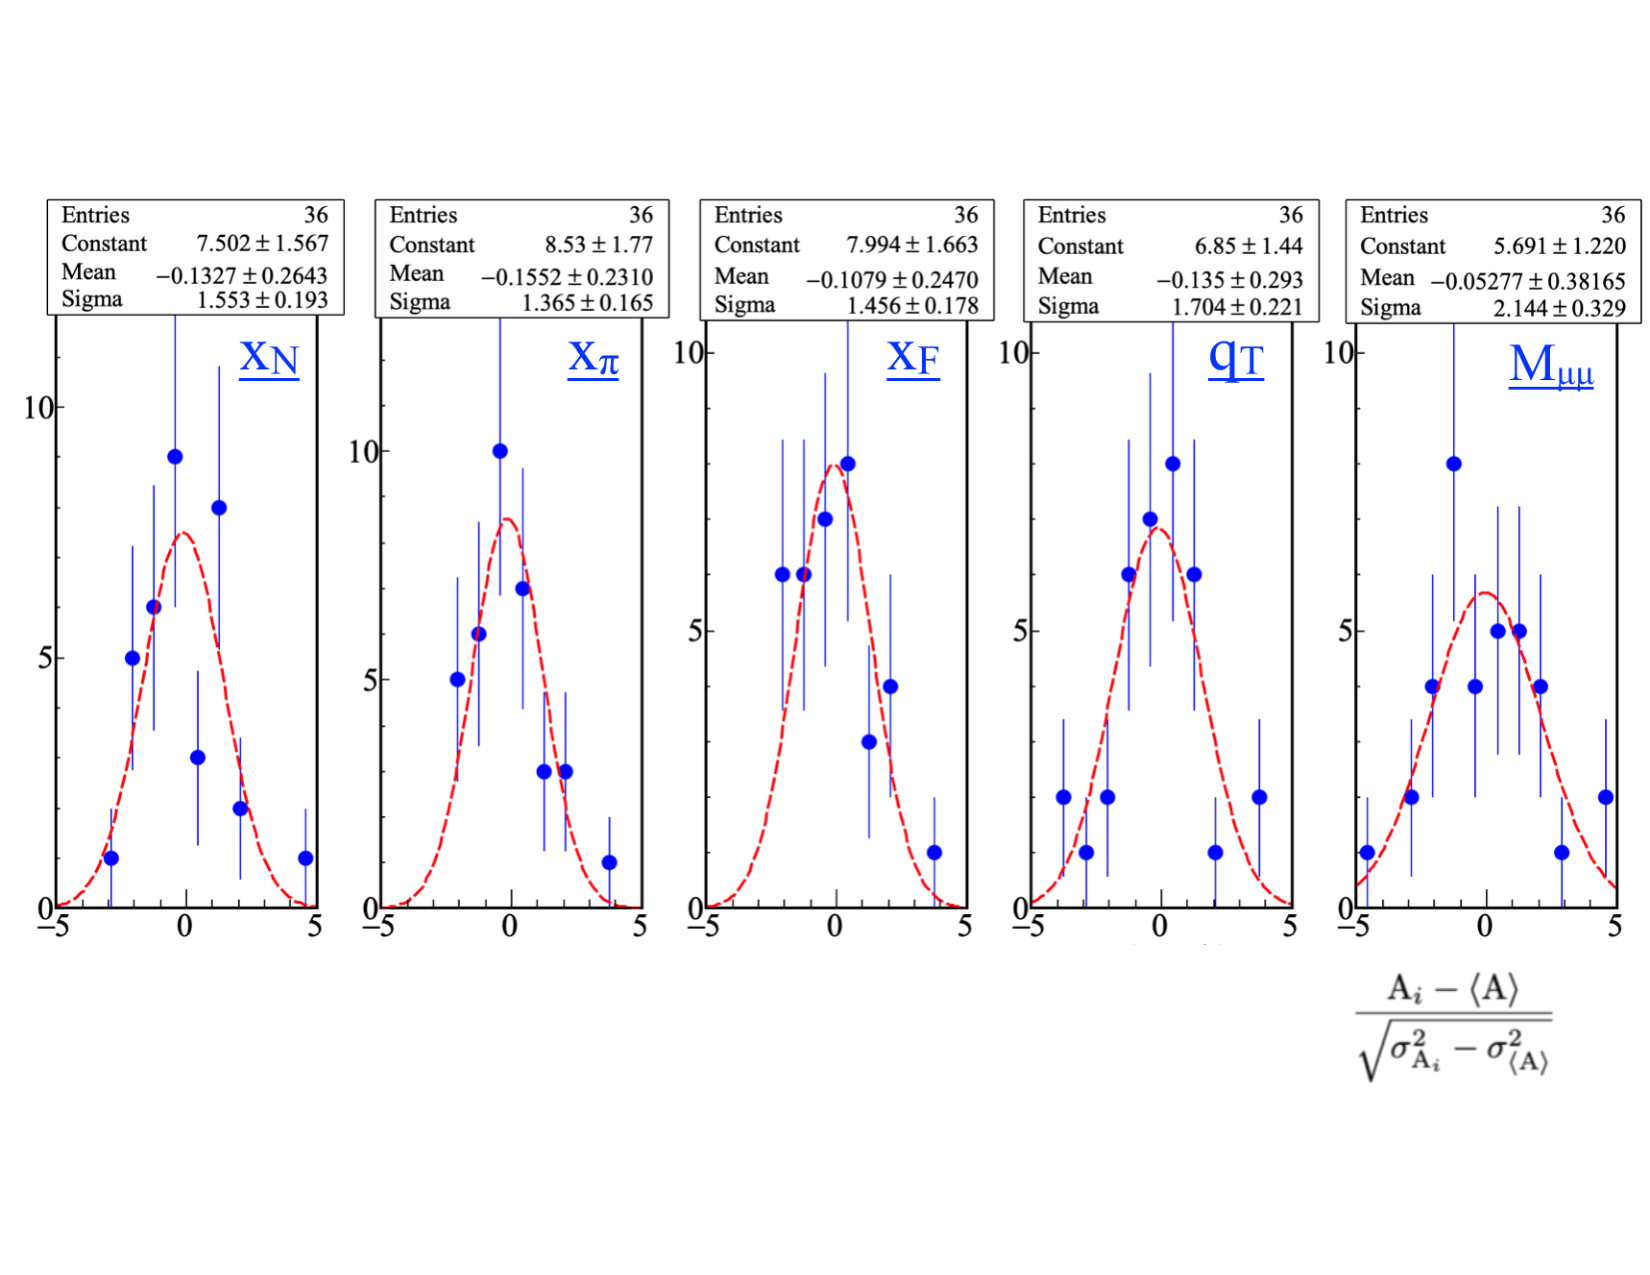
\includegraphics[width=\textwidth, trim=0cm 3cm 0cm 3cm,
    clip]{faPullsUpSJPsi}
  \caption{Pull distributions from the false asymmetry in the upstream target
    cell}
  \label{fig::faPullsUpSJPsi}
  \end{figure}

\begin{figure}[h!t]
  \centering 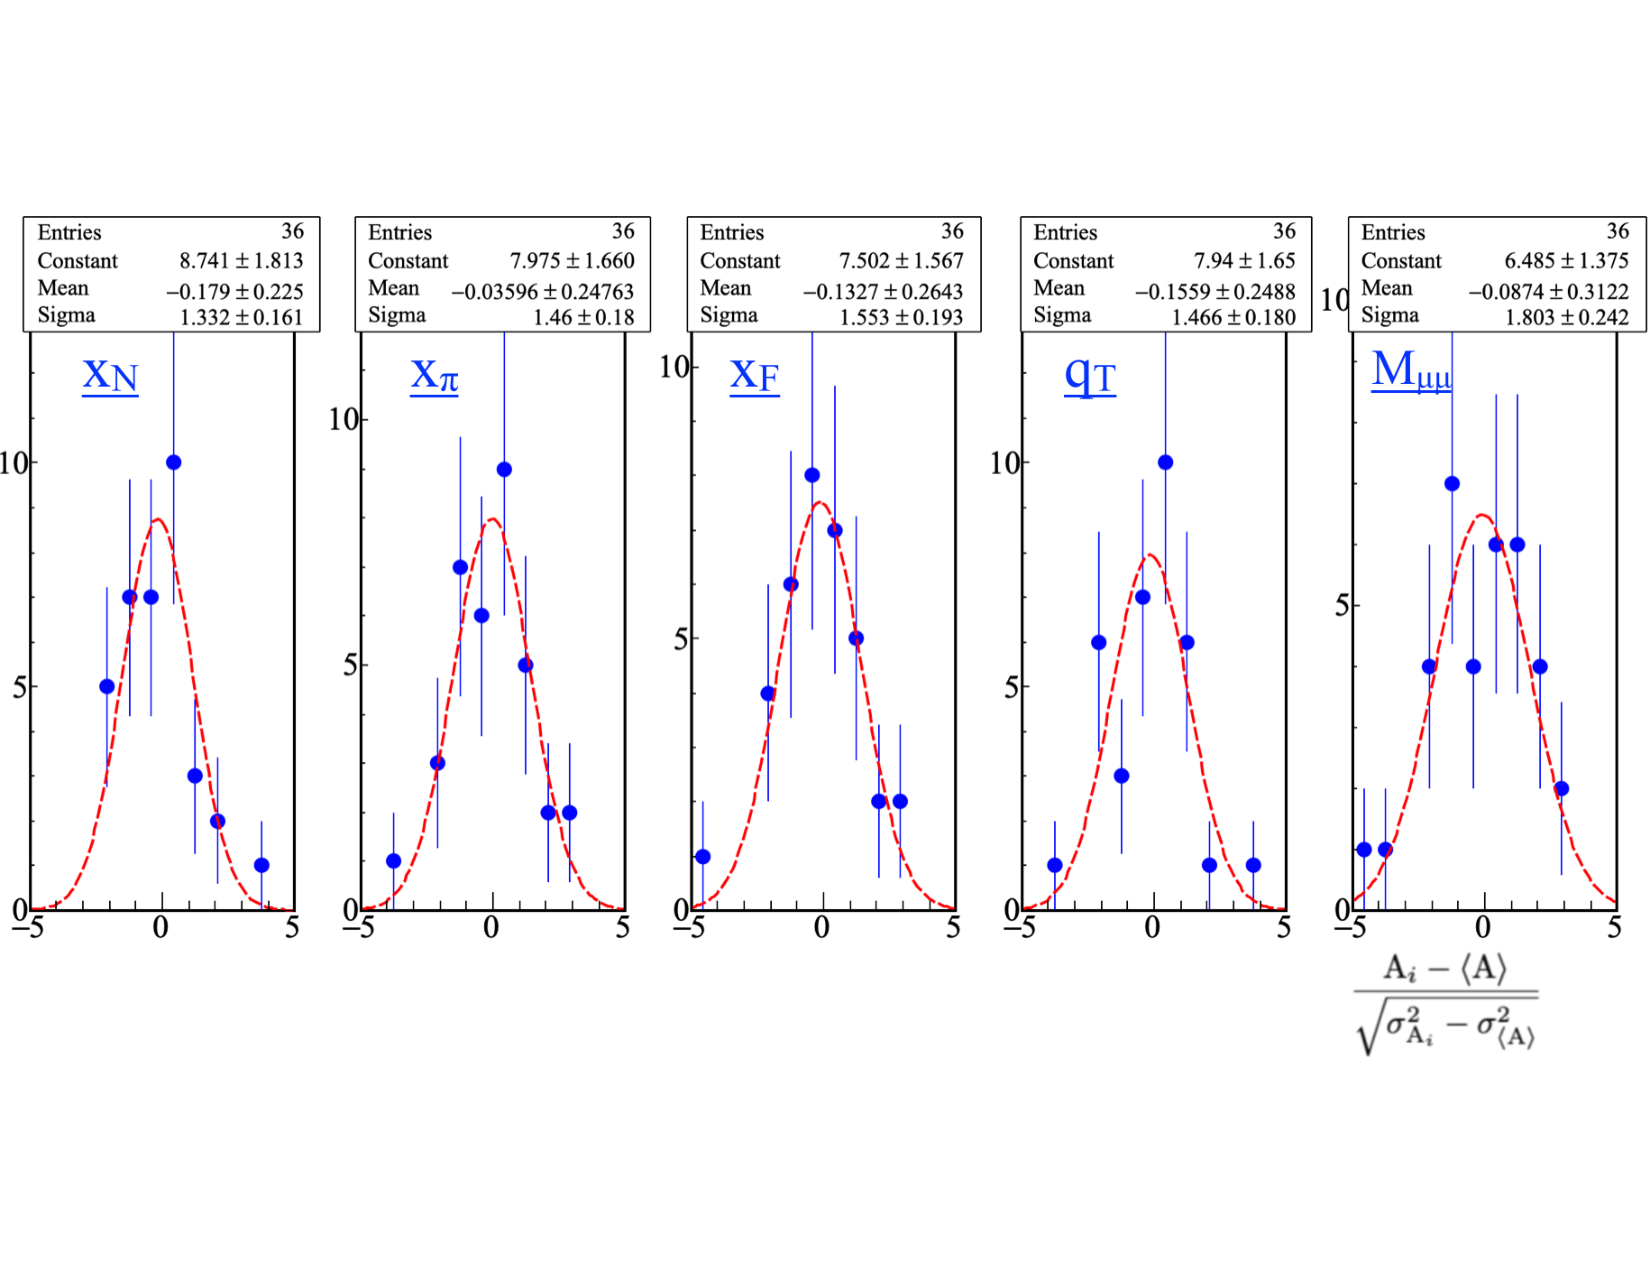
\includegraphics[width=\textwidth, trim=0cm 3cm 0cm 3cm,
    clip]{faPullsDownSJPsi}
  \caption{Pull distributions from the false asymmetry in the downstream target
    cell}
  \label{fig::faPullsDownSJPsi}
\end{figure}

\end{enumerate}

The systematic error from each false asymmetry is determined using the
Eq.~\ref{equ::sysErrorPullJPsi}.  The uncorrelated pulls have only 4 (number of
bins) $\times$ 9 (number of periods) = 36 entries which results in large errors
on the Gaussian fit results.  In an attempt to correct for this and to take into
account the fit errors, a weighted average of the mean and standard deviation is
made using the fit parameters and fit errors as weights from the uncrrelated
pull distributions.  This is the same technique as was used to determine the
systematic error from fluctuations in time.  The resulting weighted mean and
weighted standard deviation are then used to calculate the systematic error.  A
summary of the systematic error from each false asymmetry is shown in
Table~\ref{tab::faSysJPsi}.  The systematic error due to additional factors is
chosen as the largest systematic error from Table~\ref{tab::faSysJPsi}.

\begin{table}[h!t]
  \centering
  \begin{tabular}{|c|c|}
    \hline Systematic error& \multirow{2}{9em}{$\langle
      \sigma_{\mathrm{systematic}}/\sigma_{\mathrm{statistical}}
      \rangle$}\\ & \\ \hline

    Two target acceptance estimation& 0.19\\ \hline
    
    Target Cell 1& 1.20\\ \hline

    Target Cell 2& 1.11\\ \hline
    
  \end{tabular}
  \caption{Summary of systematic error impacts from false asymmetries changes in
    time.  The maximum systematic error is chosen as the systematic error.}
  \label{tab::faSysJPsi}
\end{table}

\subsubsection{Total Systematics}
The total systematic error is determined by adding all systematic errors in
quadrature as

\begin{equation}
  \Big \langle \frac{
    \sigma_{\mathrm{systematic}}}{\sigma_{\mathrm{statistical}}} \Big \rangle =
  \sqrt{ \sum_i^{\mathrm{all \; systematic}} \Big \langle
    \frac{\sigma^2_{\mathrm{systematic, i}}}{\sigma^2_{\mathrm{statistical}}}
    \Big \rangle } \;,
\end{equation}
where all the systematic effects considered are summarized in
Table.~\ref{tab::sysErrorJPsi}.  For reference the total statistical error is
$\langle \sigma_{\mathrm{statistical}} \rangle$ = 0.006.

\begin{table}[h!t]
  \centering
  \begin{tabular}{|c|c|c|}
    \hline
    \multirow{2}{*}{Systematic error}&
    \multirow{2}{*}{
      $\langle \sigma_{\mathrm{systematic}}/\sigma_{\mathrm{statistical}}
      \rangle$} &
    \multirow{2}{*}{$\langle \sigma_{\mathrm{systematic}} \rangle$}\\
    & & \\ \hline \hline

    Period compatibility& 0.16& 0.001\\ \hline

    Left-Right migration& 0.044& 0.0003\\ \hline

    J/$\Psi$ purity& 0.095& 0.0006\\ \hline

    Target Polarization& 0.05& 0.0003\\ \hline

    Dilution Factor& 0.05& 0.0003\\ \hline

    Acceptance fluctuation& 0.23 & 0.001\\ \hline

    False asymmetry& 1.2 & 0.008\\ \hline \hline
    \textbf{Total}& \textbf{1.24} & \textbf{0.008}\\\hline
    
  \end{tabular}
  \caption{Summary of systematic error impacts to the integrated asymmetry}
  \label{tab::sysErrorJPsi}
\end{table}

The integrated left-right asymmetry result and systematic error band is shown in
Fig.~\ref{fig::Alr_JPsi} and the kinematic dependencies are shown in
Fig.~\ref{fig::AlrBinned_JPsi}.  Similarly to the left-right asymmetry for the
high mass Drell-Yan analysis, the integrated left-right asymmetry is 1 sigma
above zero.  The asymmetry shows a weak inverse dependence on $x_F$ indicating
the asymmetry could be related to quark distributions in the proton target.
This can also be seen in the $x_N$ dependence which is most significant in the
highest $x_N$ bin.  Although the left-right asymmetry is model independent, it
is was discussed that the Sivers function could be the cause of for a non-zero
left-right asymmetry.  A positive left-right asymmetry would be consistent with
the sign change hypothesis.

\begin{figure}[h!t]
  \centering
  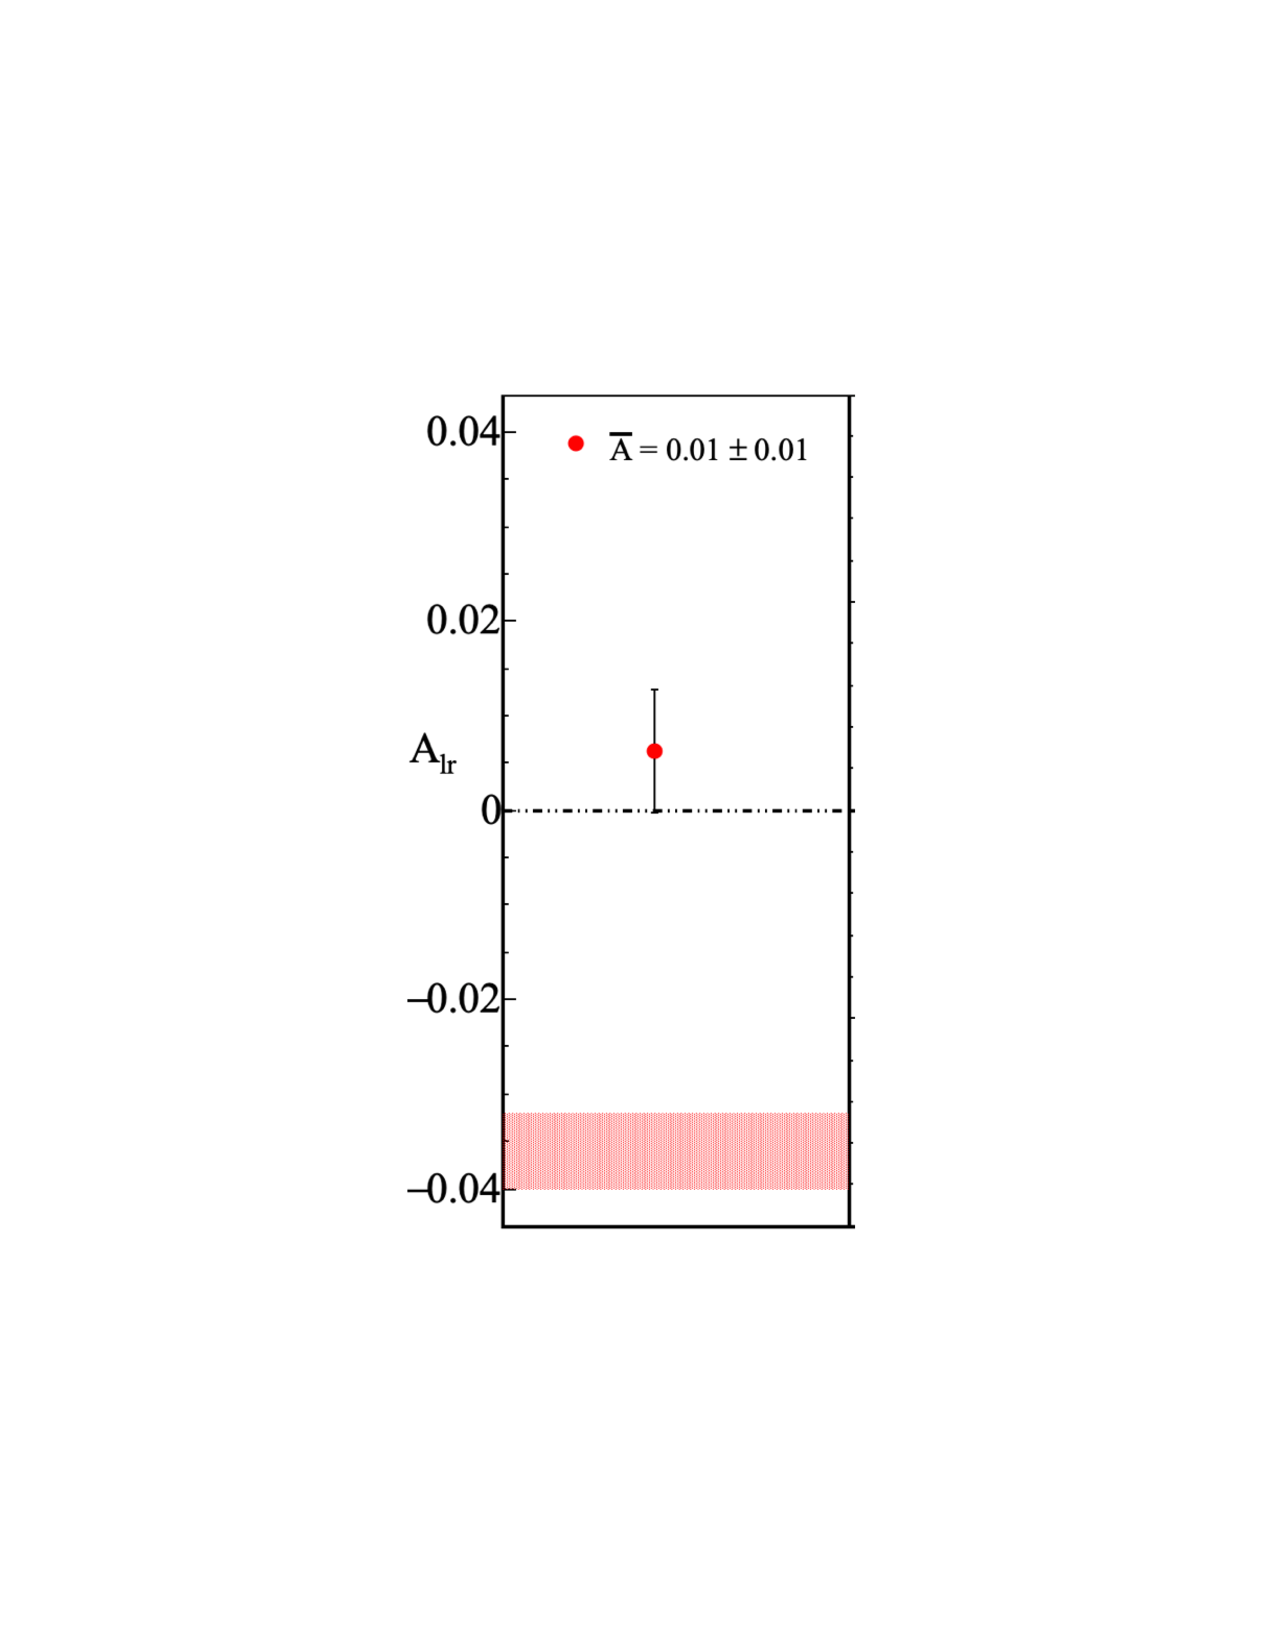
\includegraphics[width=0.2\textwidth,trim=6cm 6cm 6cm 6cm,clip]{Alr_JPsi}
  \caption{The integrated left-right asymmetry from the mass range
    2.87-3.38~{\gvcw}.  The systematic error bands are shown in red at the
    bottom of the plot.}
  \label{fig::Alr_JPsi}
\end{figure}

\begin{figure}[h!t]
  \centering 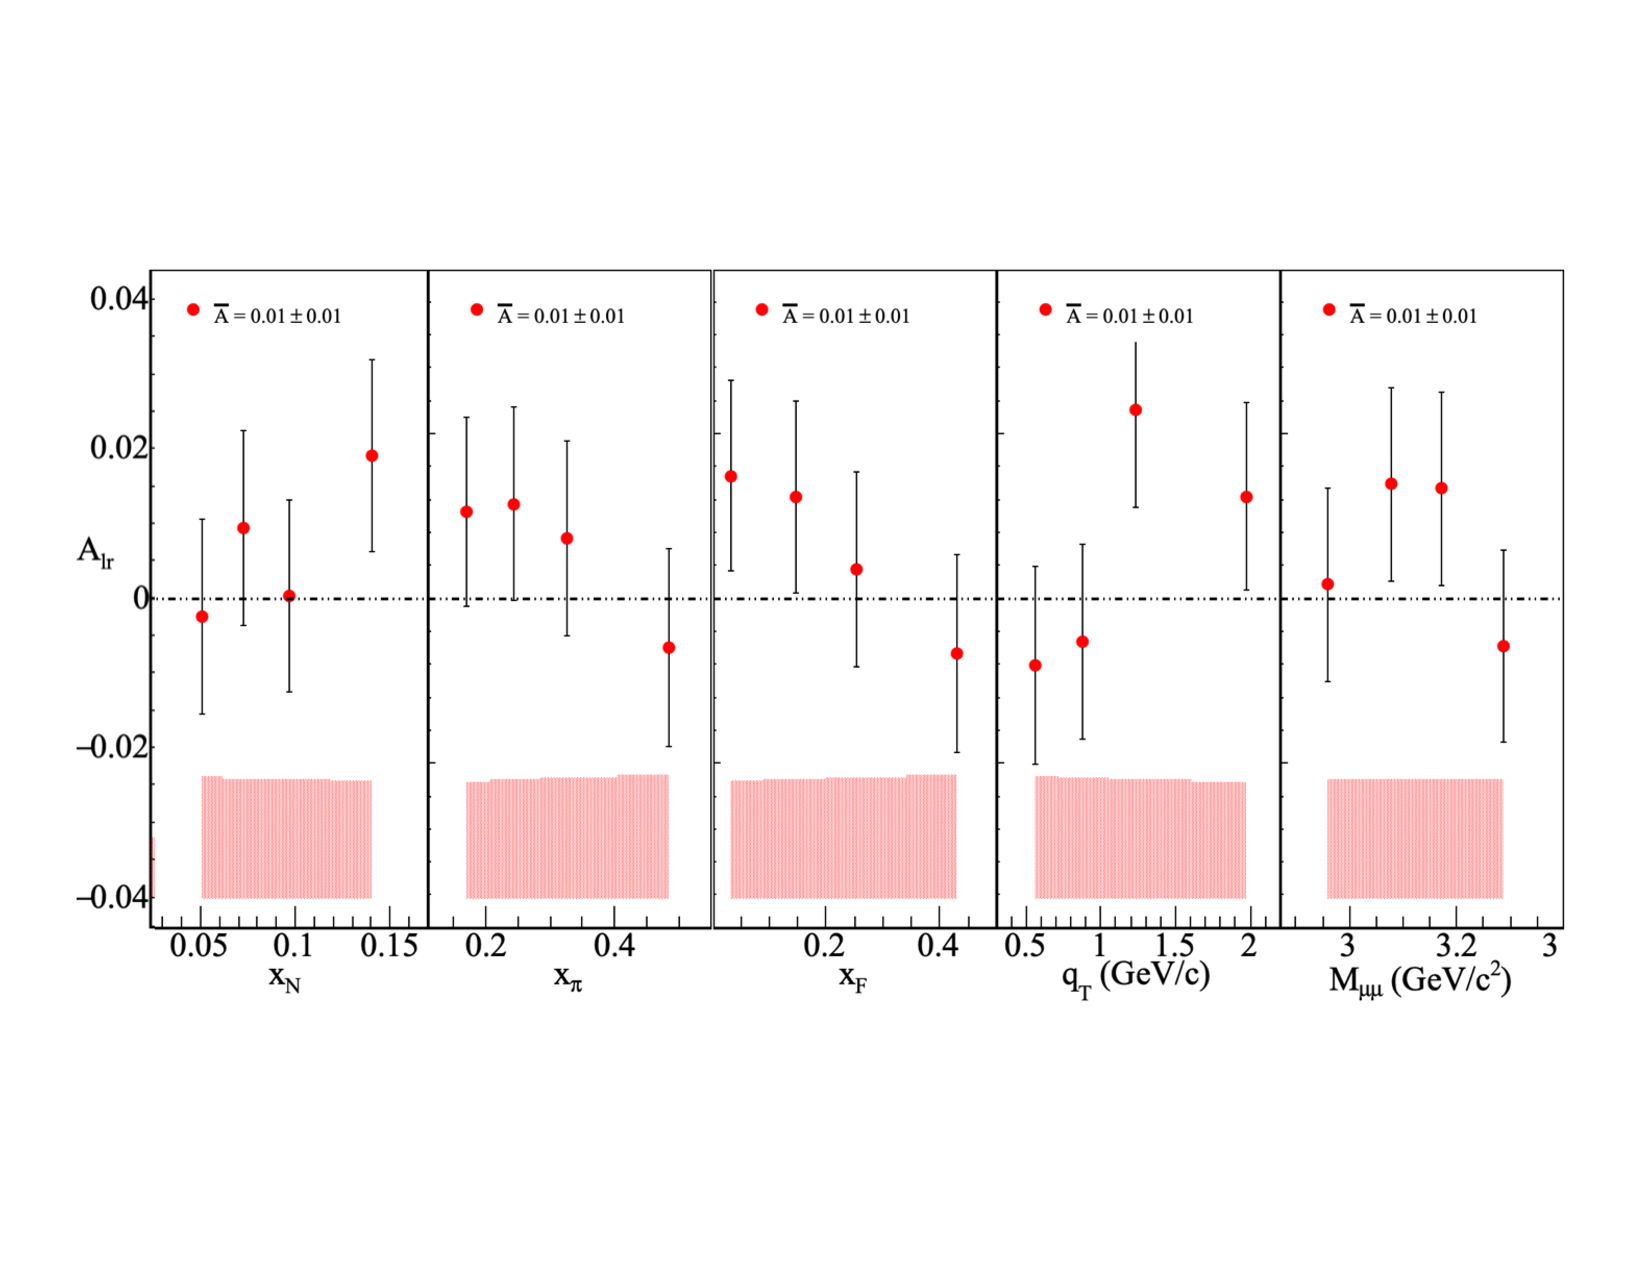
\includegraphics[width=\textwidth,trim=1cm 4cm 1cm
    4cm,clip]{AlrBinned_JPsi}
  \caption{The kinematic dependencies of the left-right asymmetry from the mass
    range 2.87-3.38~{\gvcw}.}
  \label{fig::AlrBinned_JPsi}
\end{figure}

The Anselmino group derived an expression for the $A_N$ asymmetry from {\jp}
production as~\cite{Anselmino:2016fhz}

\begin{equation}
  A^{J\Psi}_{N} \propto f_{\bar{q}/H_a}(x_a, k_{aT})
  \frac{k_{bT}}{M_b} \otimes f_{1T}^{\perp q}(x_b, k_{bT}),
\end{equation}
\noindent
and a made predictions for the $A_N$ asymmetry as a function of $x_N$ and $q_T$
shown in Fig.~\ref{fig::AN_JPsiPredict}.  As derived in
Sec~\ref{sec::lr_theory}, $A_{N} = \frac{\pi A_{lr}}{2}$.  More details are
given in Sec~\ref{sec::theory_jpsi}, but their calculation assumed the dominant
contribution to {\jp} production is from quark-quark annihilation.
Fig.~\ref{fig::AN_JPsi} shows the results determined at COMPASS for the $A_N$
asymmetry determined by modifying the left-right results in
Fig.~\ref{fig::AlrBinned_JPsi}.  The maximum $A_N$ asymmetry, determined at
COMPASS, is less than 0.05 which when comparing to the prediction in
Fig.~\ref{fig::AN_JPsiPredict} is 2 sigma less than the prediction.

\begin{figure}[h!t]
  \centering 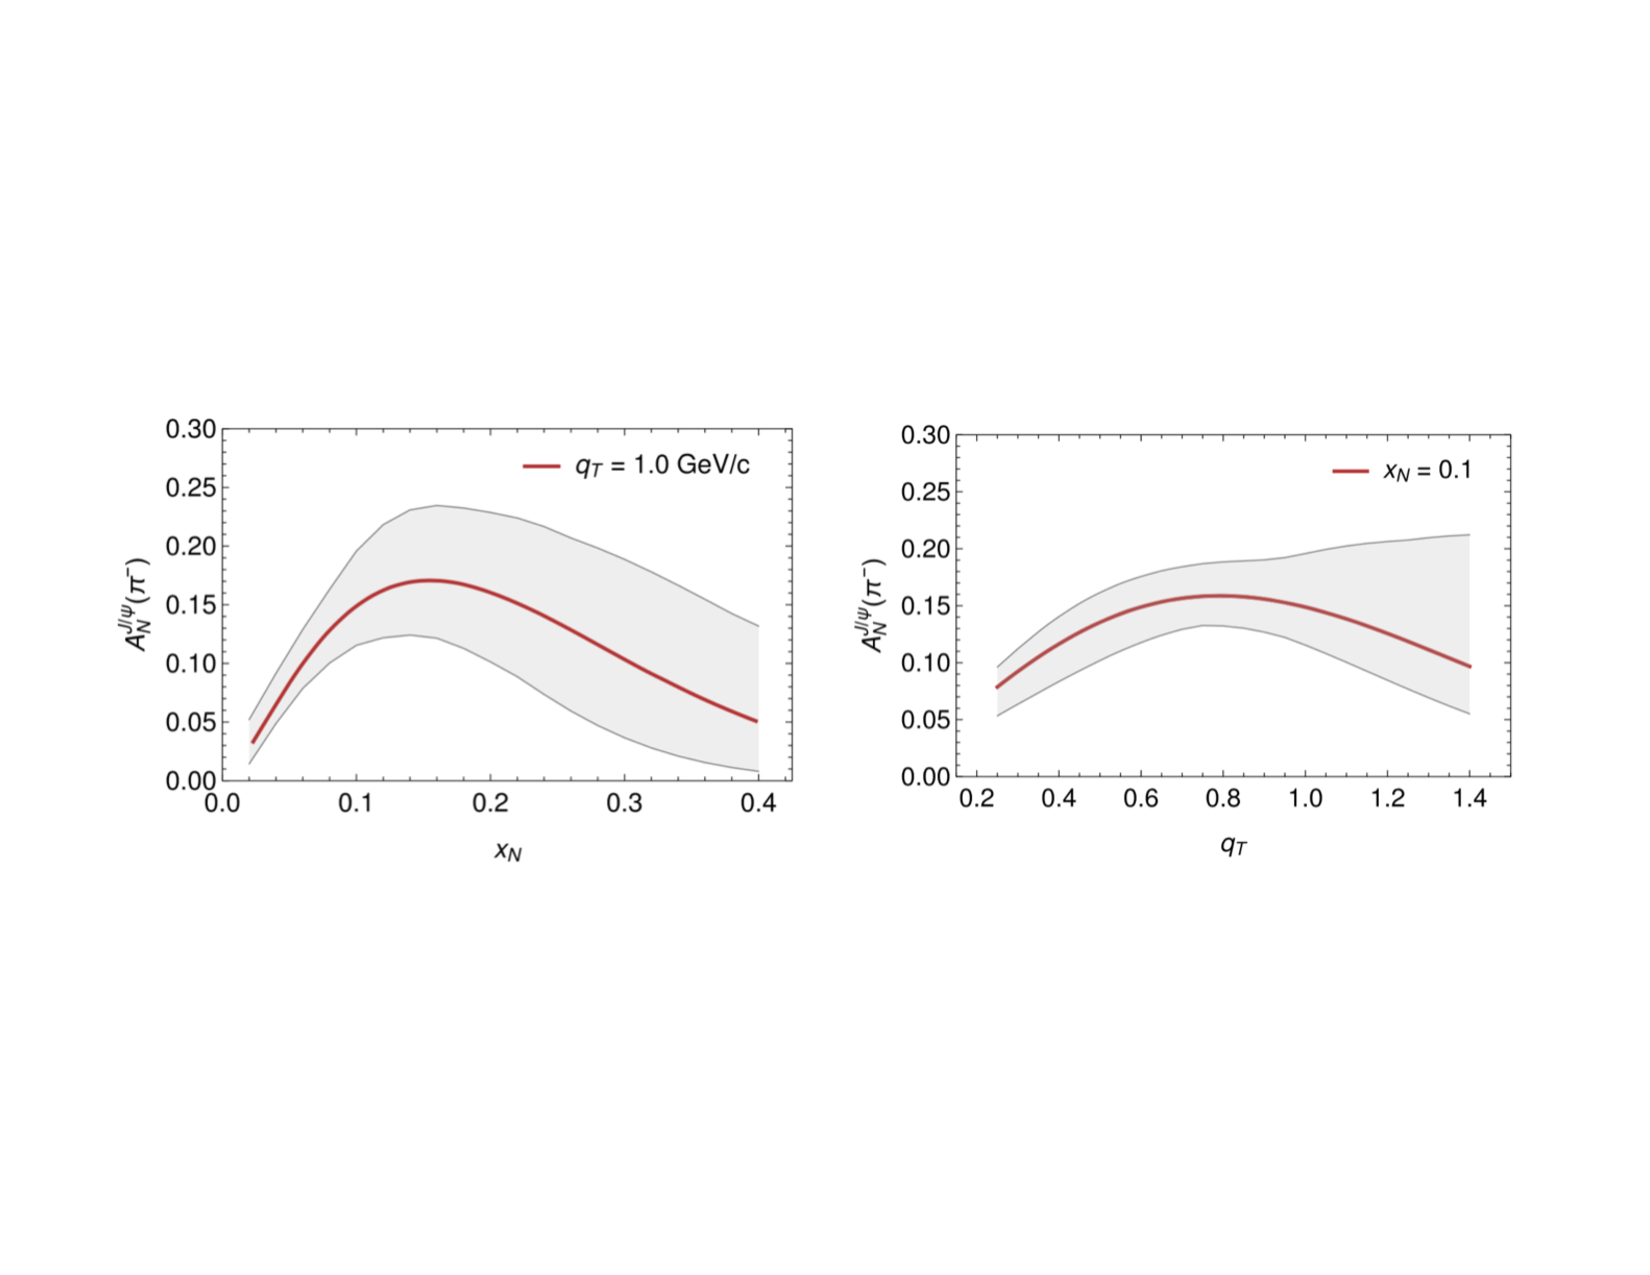
\includegraphics[width=0.6\textwidth,trim=2cm 7cm 2cm
    7cm,clip]{AN_JPsiPredict}
  \caption{Predictions for the analyzing power, $A_N$, from {\jp} production at
    COMPASS as a function of $x_N$ and $q_T$.  This image was taken
    from~\cite{Anselmino:2016fhz}.}
  \label{fig::AN_JPsiPredict}
\end{figure}

\begin{figure}[h!t]
  \centering 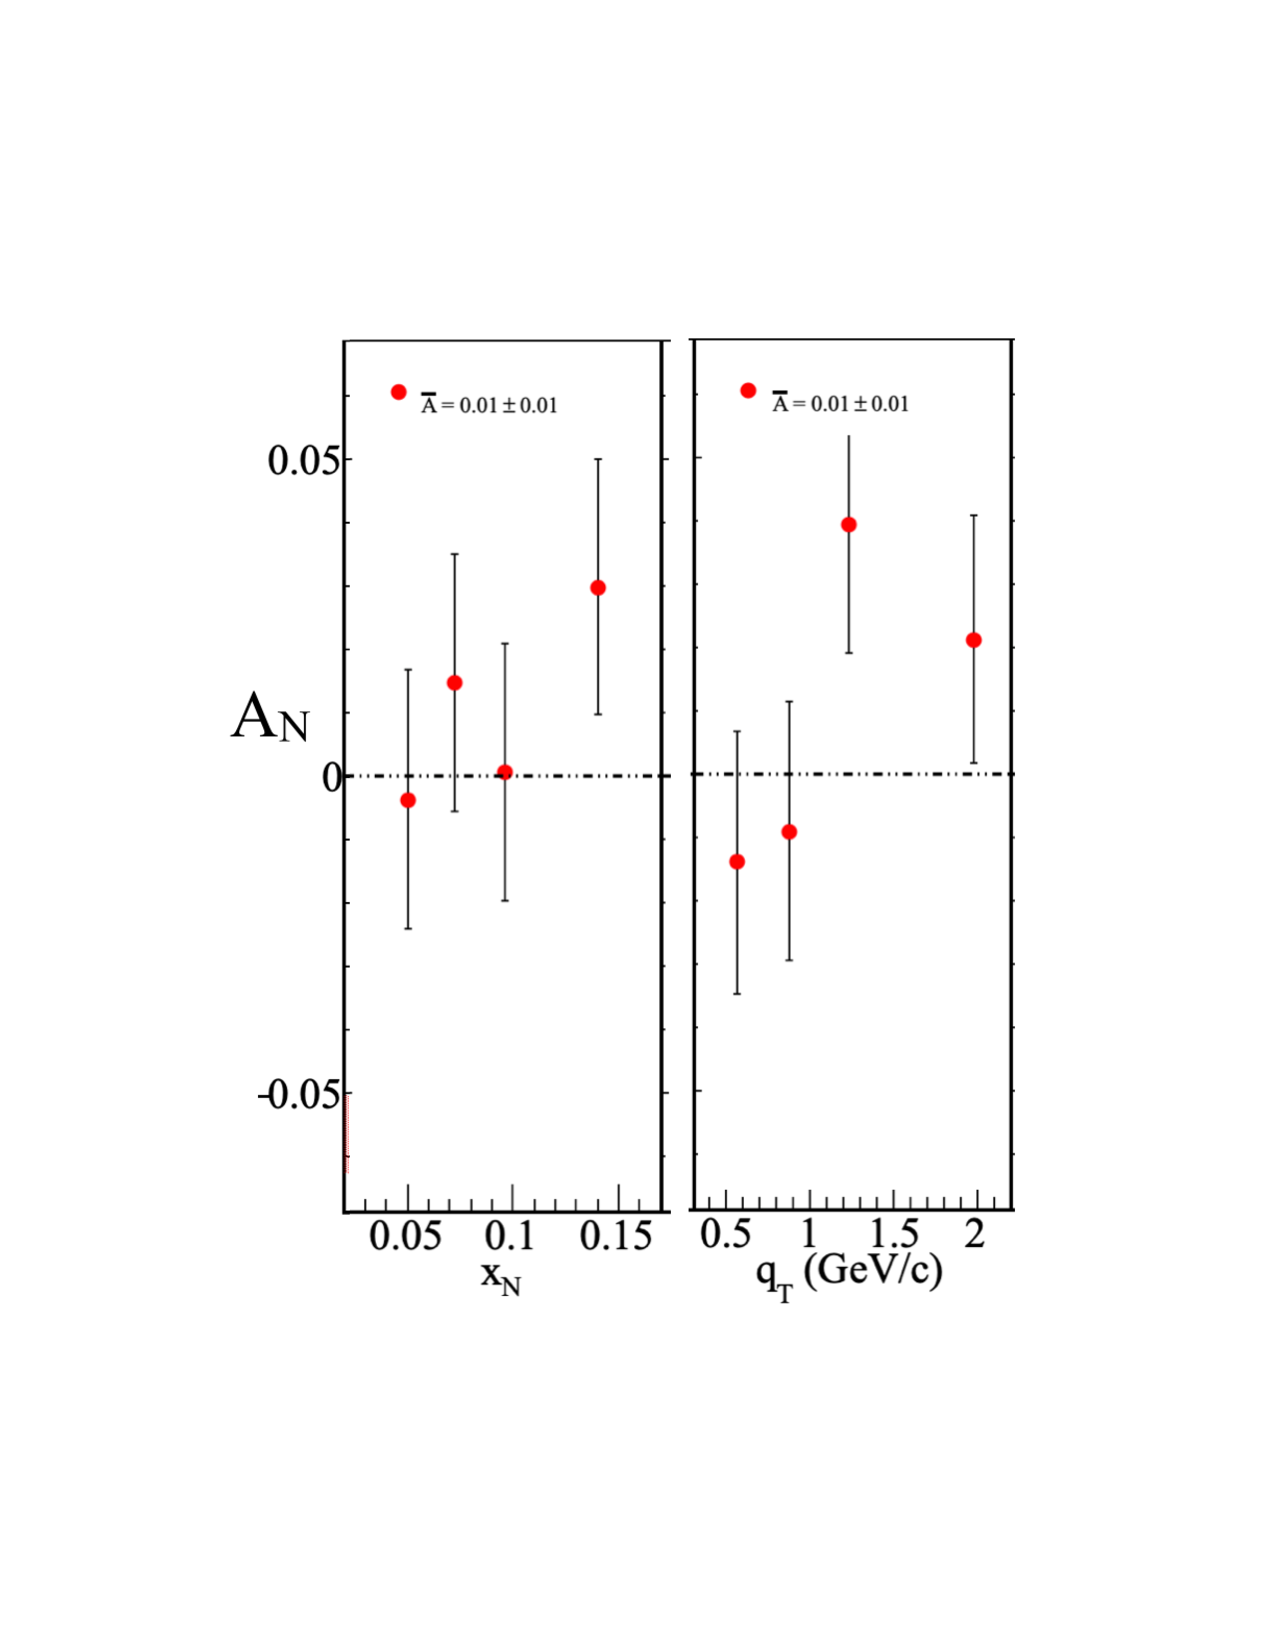
\includegraphics[width=0.3\textwidth,trim=3cm 5.5cm 3cm
    5.5cm,clip]{AN_JPsi}
  \caption{The analyzing power at COMPASS determined by modifying the left-right
    asymmetry as a function of $x_N$ and $q_T$ to be compared with the
    predictions in Fig.~\ref{fig::AN_JPsiPredict}. }
  \label{fig::AN_JPsi}
\end{figure}

The incompatibility of the theory prediction, Fig.~\ref{fig::AN_JPsiPredict},
and the results determined at COMPASS, Fig.~\ref{fig::AN_JPsi}, can be due to
either a Siver function much lower than expected or gluon-gluon fusion
contamination.  At the present moment, the Siver's function from gluon-gluon
fusion is not well known and therefore could be small or negative.
Fig.~\ref{fig::ggQQbarXsection} shows results for {\jp} production from
quark-quark annihilation and gluon-gluon fusion using the color evaporation
model~\cite{VOGT1999197}.  To determine the expected {\jp} contribution from
gluon-gluon fusion and quark-quark annihilation at COMPASS the results in
Fig.~\ref{fig::ggQQbarXsection} are weighted with the COMPASS $x_F$ distribution
in the intermediate mass range.  The determined ratio of {\jp} production from
quark-quark annihilation to gluon-gluon fusion at COMPASS is 0.8.  It is
therefore not ruled out that the results in Fig.~\ref{fig::AN_JPsi} are reduced
compared to the predictions in Fig.~\ref{fig::AN_JPsiPredict} due to gluon-gluon
fusion.

\begin{figure}[h!t]
  \centering 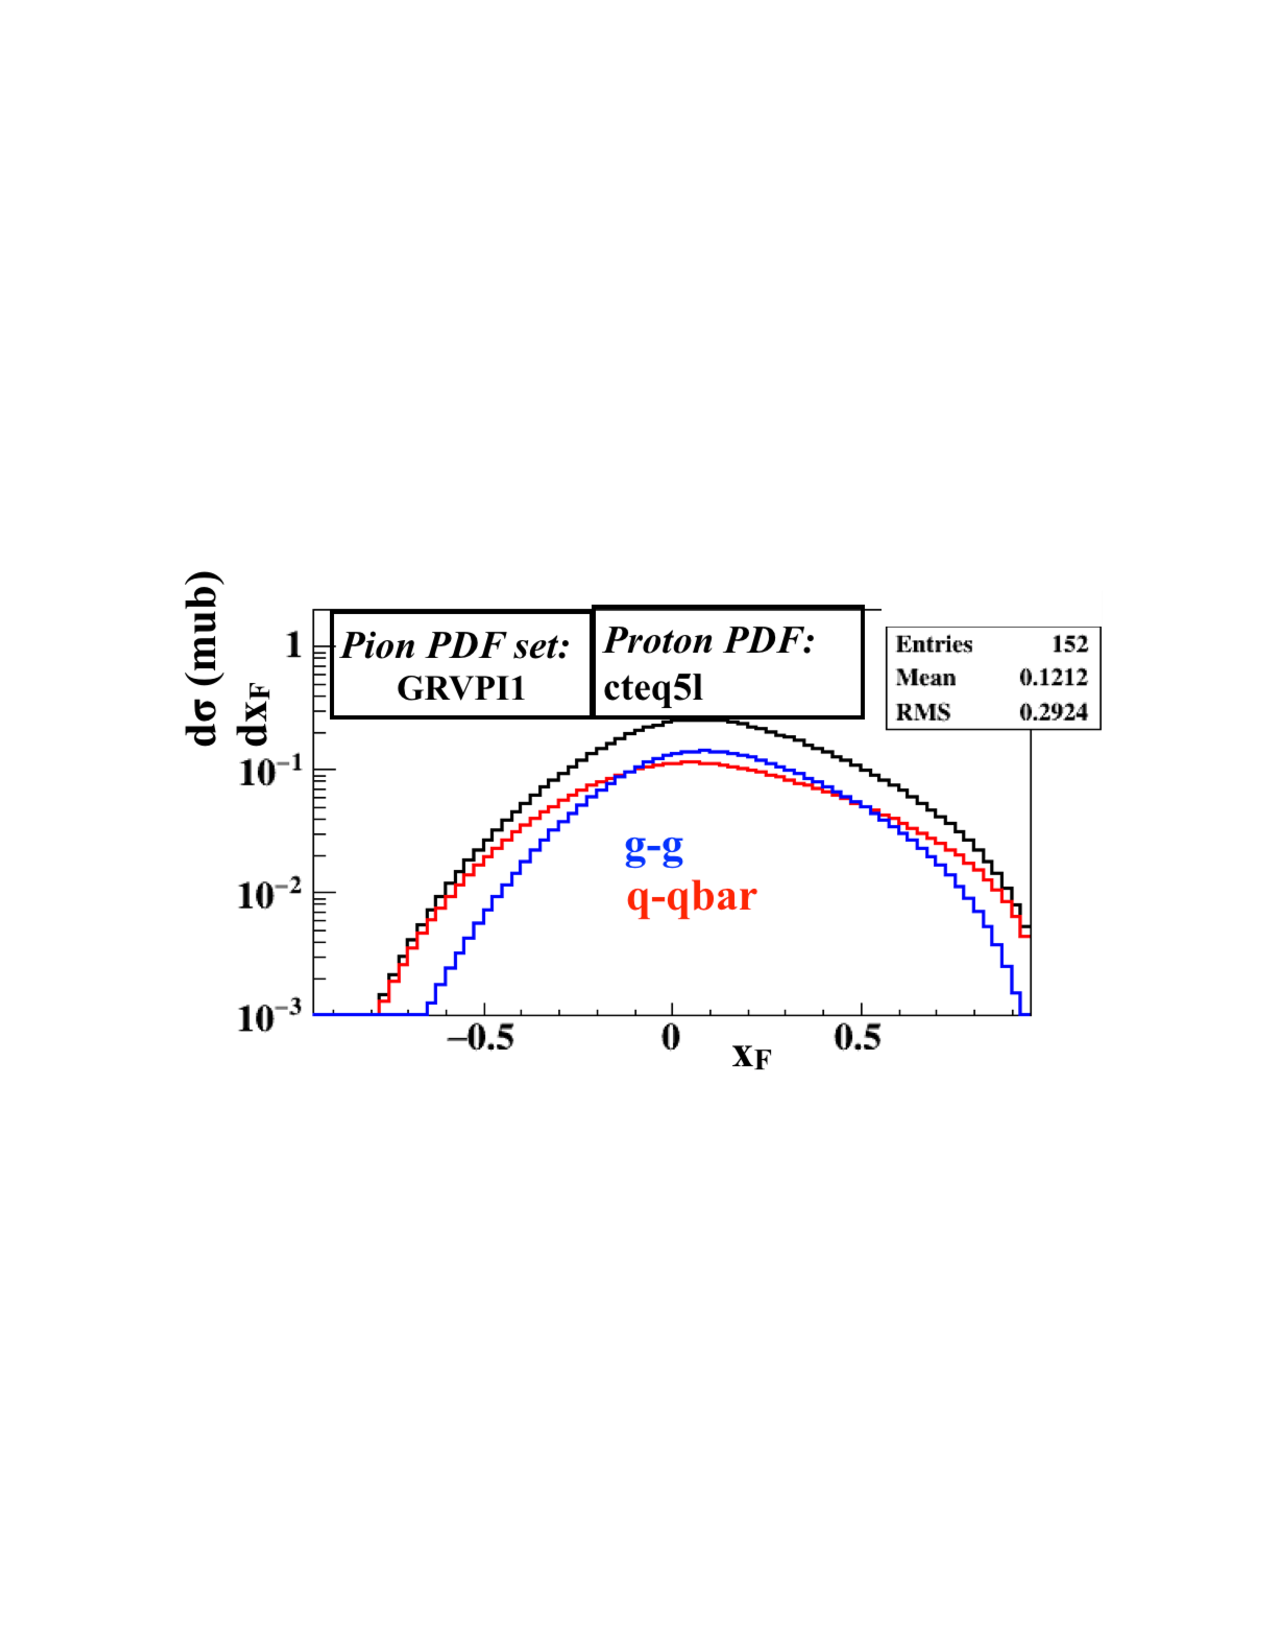
\includegraphics[width=0.55\textwidth,trim=2.5cm 9.5cm 2.5cm
    9.5cm,clip]{ggQQbarXsection}
  \caption{{\jp} production cross-section from gluon-gluon fusion (blue) and
    quark-quark annihilation (red) and the sum (black) as a function of $x_F$.
    This plot is made assuming the color evaporation model~\cite{VOGT1999197}. }
  \label{fig::ggQQbarXsection}
\end{figure}
